\shorthandoff{"}
\chapter{Forschungsergebnisse}
\label{ch:ergebnisse}

\section{Analyse von Fähigkeiten und Präferenzen}
\label{ch:ergebnisse:analyse}

\subsection{Fähigkeiten der Mitarbeiter aus dem Intranet}
\label{ch:ergebnisse:analyse:faehigkeiten}
An der Umfrage unter den Projektmitarbeitern haben N=23 Personen aus dem Fachbereich \acl{JES} der EXXETA AG teilgenommen. Diese Angestellten haben insgesamt 643 Kompetenzbewertungen im Intranet des Unternehmens abgegeben. Dies entspricht ca. 28 vergebenen Beurteilungen pro Person. Die Bewertungen verteilen sich auf 212 der \anzFaehigkeiten unterschiedlichen, im Intranet gespeicherten Fähigkeiten. Java ist mit 16 Beurteilungen die meist beherrschte Kompetenz.

Abbildung \ref{fig:ergebnisse:analyse:abb1} zeigt die im Intranet bewerteten Fähigkeiten sortiert nach Anzahl an Beurteilungen. Dabei ist der in Kapitel \ref{ch:empfehlungssysteme:cf:speicherbasiert} vorgestellte lange (Ratten-)Schwanz gut erkennbar. Dieser ist jedoch weniger stark ausgeprägt, als in der Referenzdarstellung aus Abbildung \ref{fig:empfehlungssysteme:cf:speicherbasiert:abb1}.

\begin{figure}[h]
	\centering
	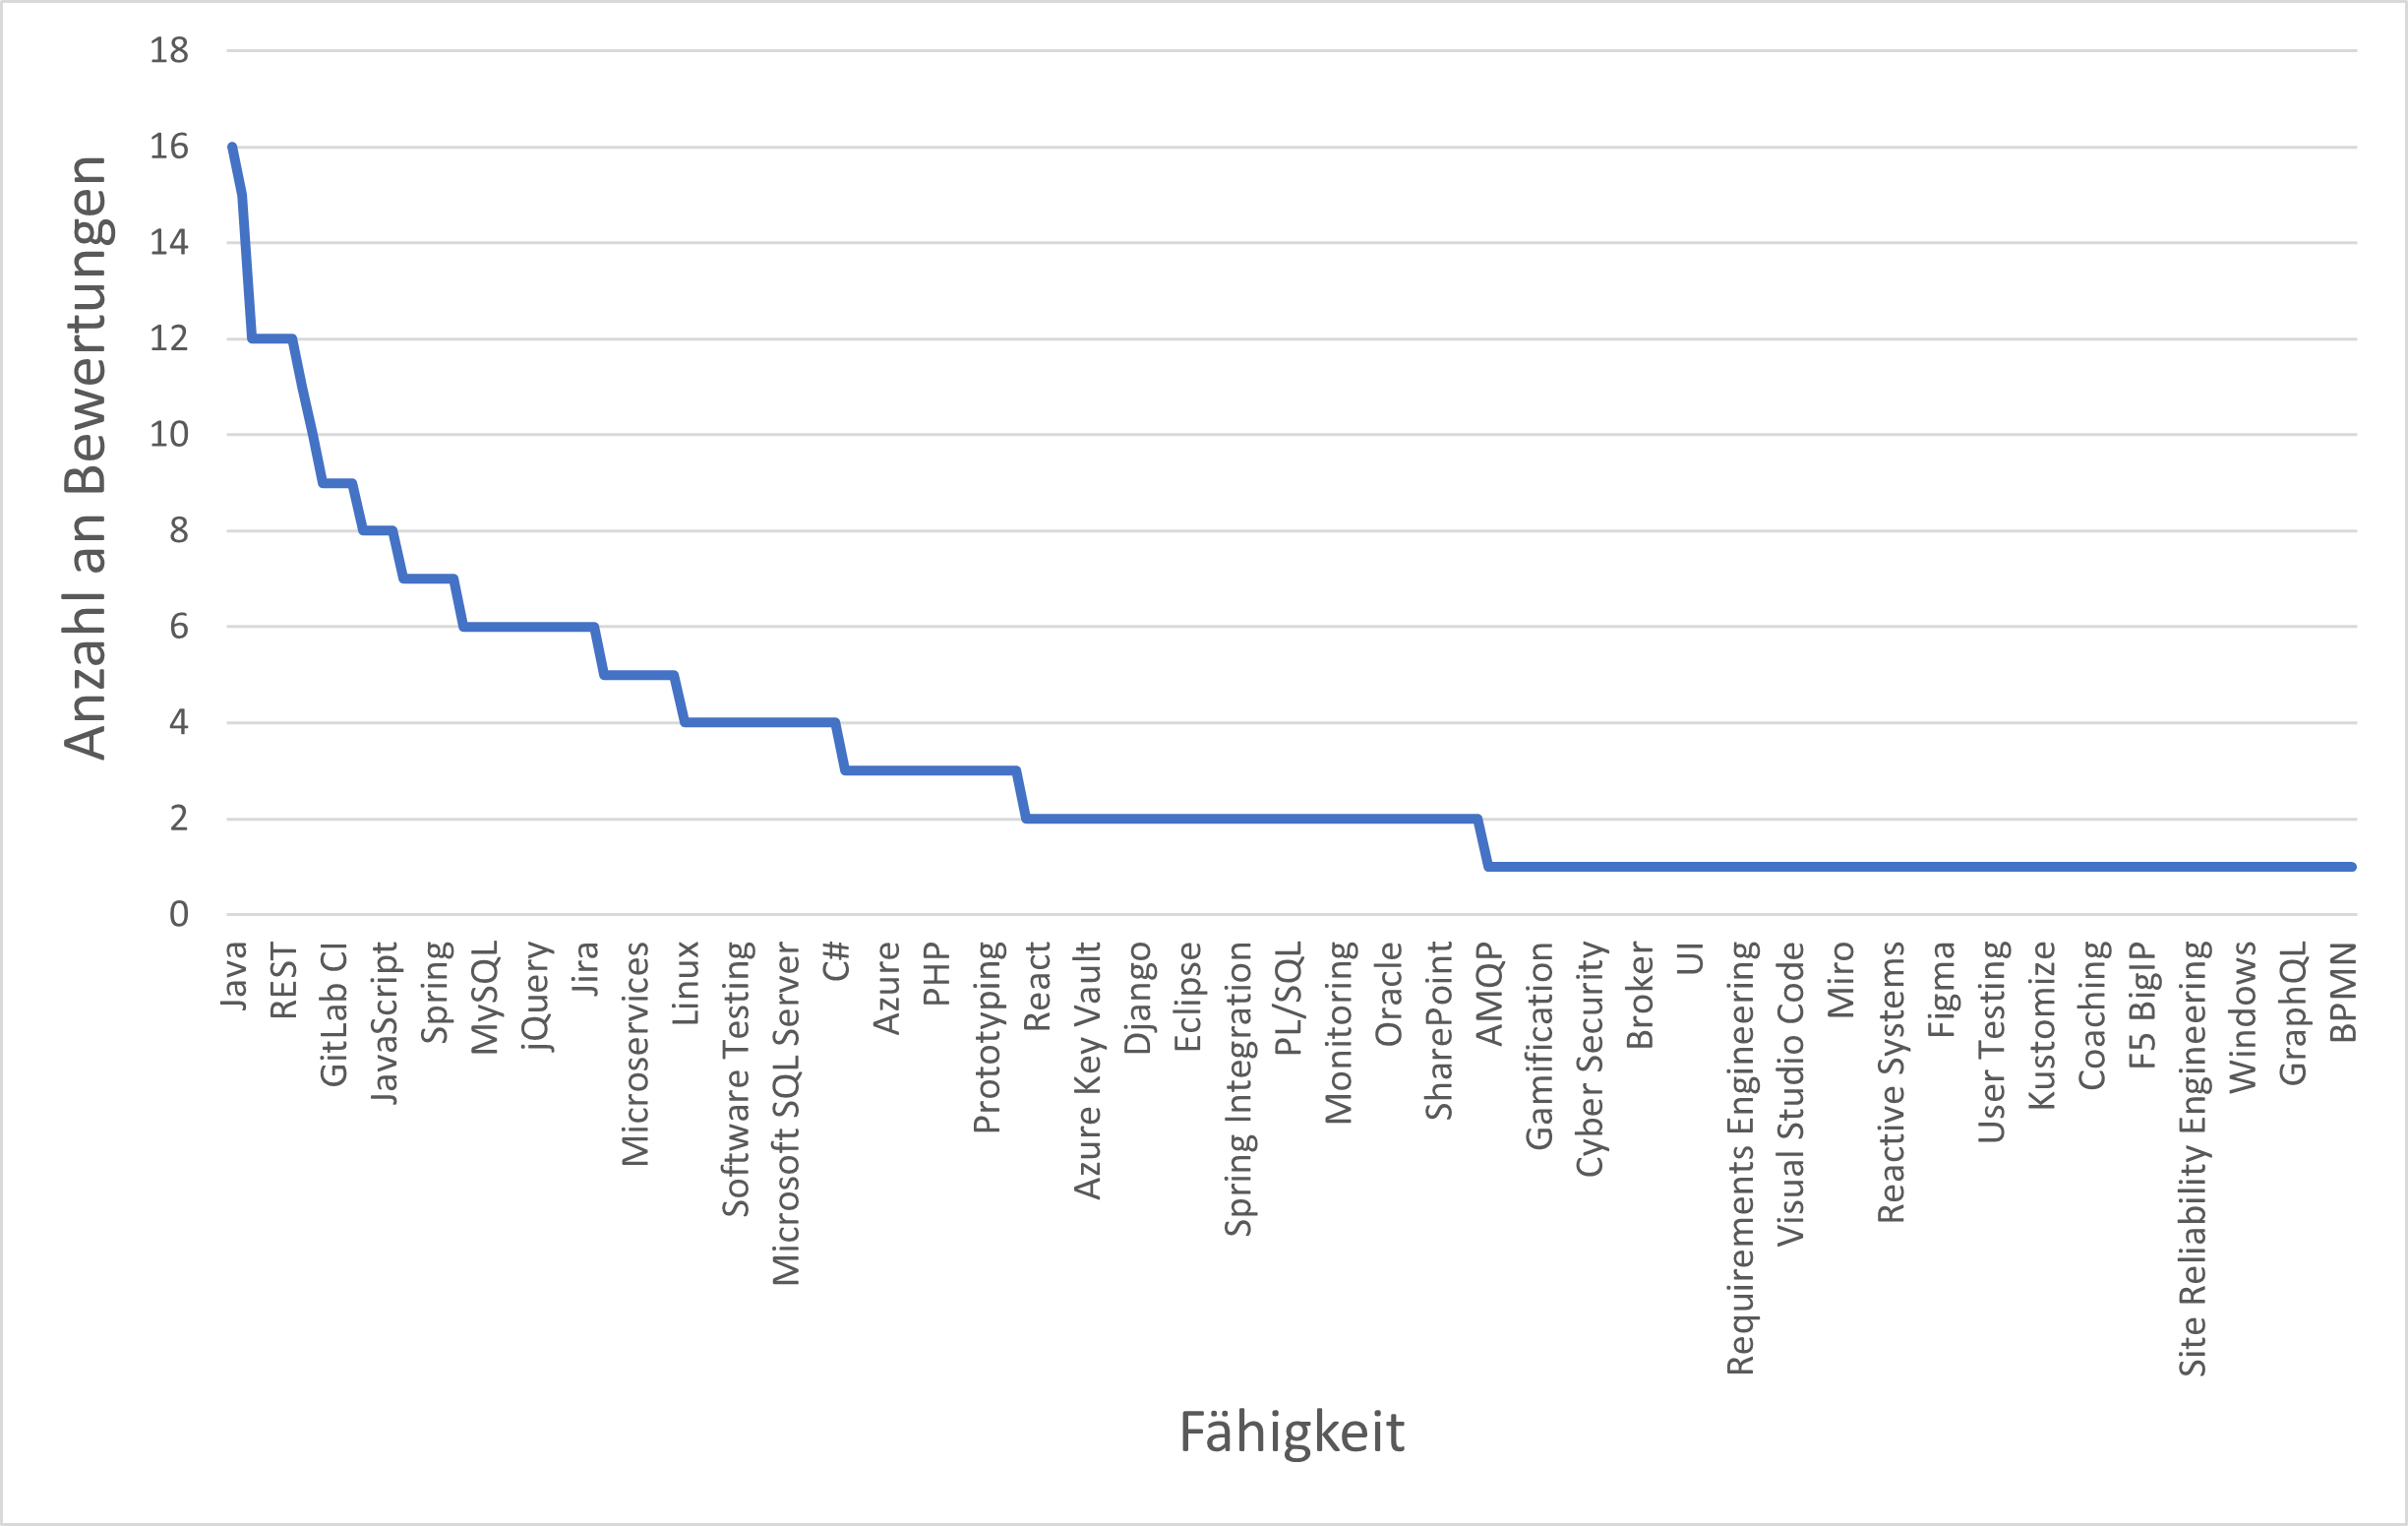
\includegraphics[width=1\textwidth]{gfx/long-tail-intranet.png}
	\caption{Langer (Ratten-)Schwanz bei den Fähigkeitsbewertungen im EXXETA-Intranet}
	\label{fig:ergebnisse:analyse:abb1}
\end{figure}

In Abbildung \ref{fig:ergebnisse:analyse:abb1} ist bezüglich des langen (Ratten-)Schwanzes festzustellen, dass neun bzw. etwa 4.3 Prozent aller Fähigkeiten über zehn oder mehr Bewertungen verfügen. Dagegen haben 151 bzw. etwa 71.2 Prozent aller Kompetenzen drei oder weniger Beurteilungen.

In den vorliegenden Daten des Intranets ist darüber hinaus zu beobachten, dass vier bzw. etwa 17.4 Prozent der Mitarbeiter keine einzige Fähigkeit bewertet haben. Diese Angestellten sind seit Einführung des Kompetenz-Bewertungssystems durchgehend in einem Projekt tätig und daher von ihrer Führungskraft noch nicht zur Pflege ihrer Fähigkeiten aufgefordert worden.

\subsection{Präferenzen der Mitarbeiter aus der Umfrage}
\label{ch:ergebnisse:analyse:praeferenzen}
Bei der Umfrage zu den Präferenzen haben die Mitarbeiter insgesamt 1408 Bewertungen abgegeben, welche sich auf 370 einzelne Kompetenzen verteilen. Dies entspricht knapp über 61 abgegebenen Wünschen pro Mitarbeiter. Git ist mit 18 Beurteilungen die meist präferierte Fähigkeit. Wie in Abbildung \ref{fig:ergebnisse:analyse:abb2} zu erkennen, deutet sich auch hinsichtlich der Wünsche ein langer (Ratten-)Schwanz an, wenn die Fähigkeiten nach Anzahl an Beurteilungen sortiert dargestellt werden.
 
\begin{figure}[h]
	\centering
	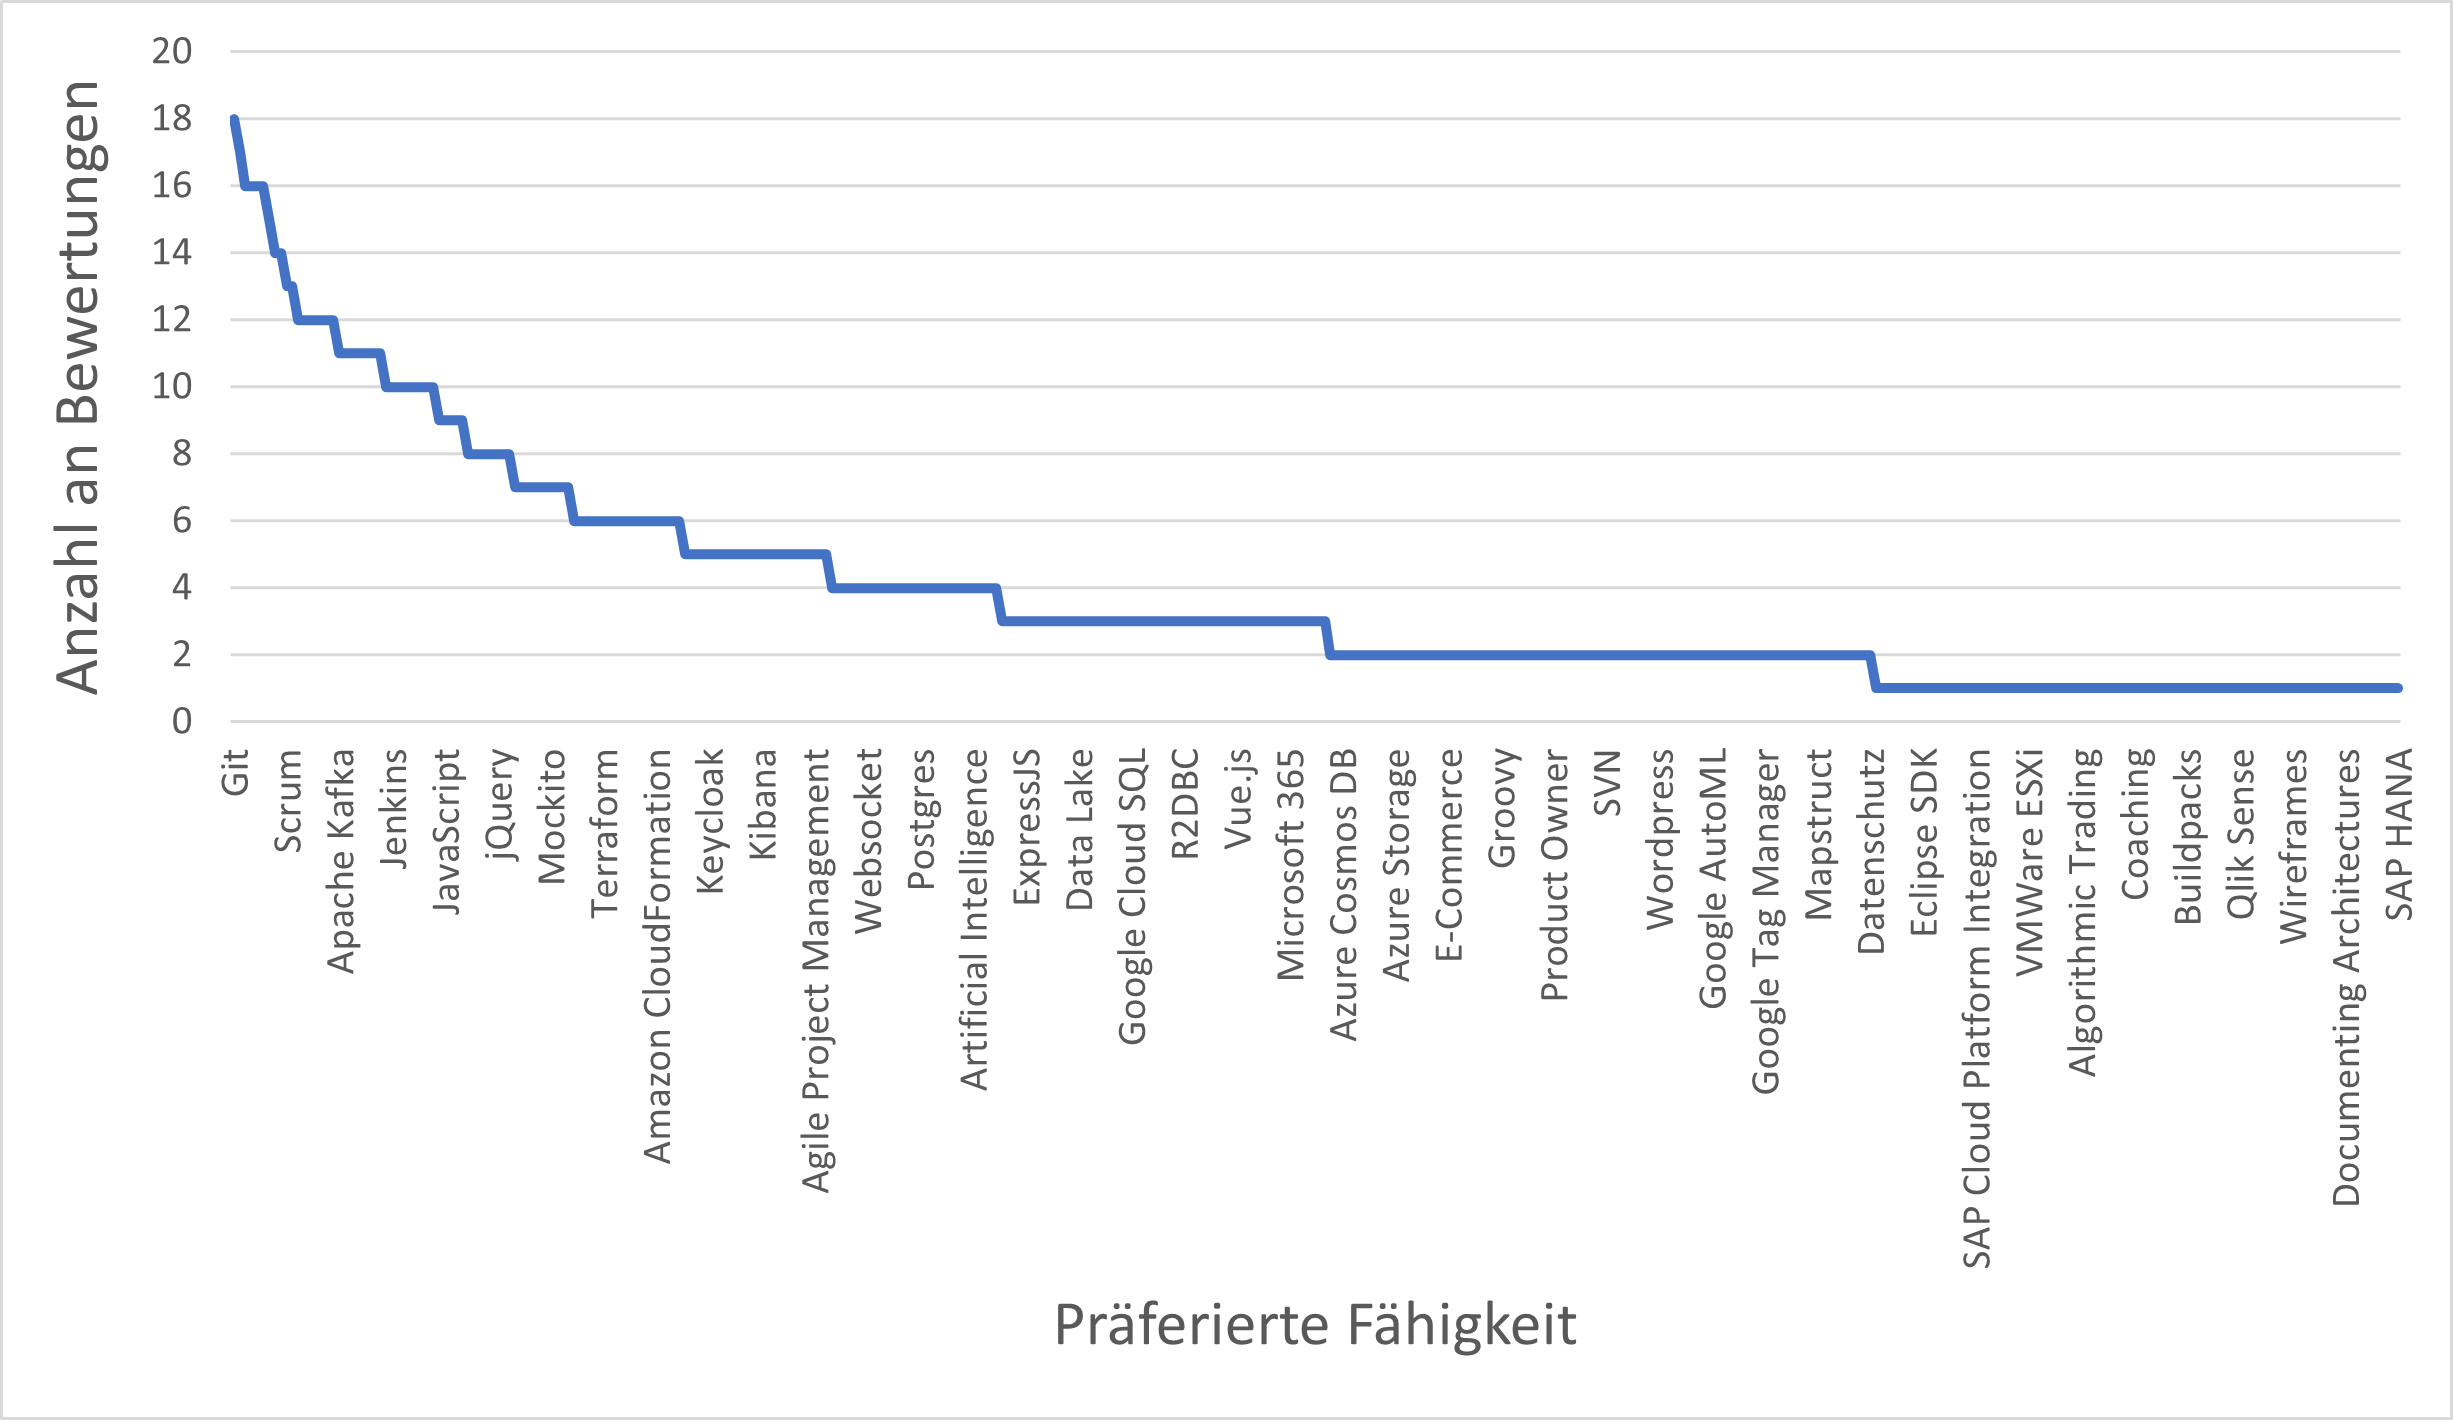
\includegraphics[width=1\textwidth]{gfx/long-tail-praeferenzen.png}
	\caption{Langer (Ratten-)Schwanz bei den präferierten Fähigkeiten der Mitarbeiter}
	\label{fig:ergebnisse:analyse:abb2}
\end{figure}

Zu Abbildung \ref{fig:ergebnisse:analyse:abb2} ist festzustellen, dass 18 bzw. etwa 4.9 Prozent aller Fähigkeiten von zwölf oder mehr Mitarbeitern präferiert werden. Dem gegenüber stehen 268 bzw. etwa 72.4 Prozent aller Kompetenzen, welche vier oder weniger Angestellte als Wunsch angegeben haben. Bei der Umfrage gab es keinen Mitarbeiter, welcher keine einzige Fähigkeit als Präferenz ausgewählte.

\subsection{Gemeinsame Betrachtung beherrschter und präferierter Fähigkeiten}
\label{ch:ergebnisse:analyse:gemeinsam}
Bei der gemeinsamen Betrachtung von Kompetenzen und Wünschen ist auf Mitarbeiterebene festzustellen, dass ein durchschnittlicher Angestellter etwa 74.7 Fähigkeiten beherrscht und/oder präferiert. Abbildung \ref{fig:ergebnisse:analyse:abb3} zeigt, wie viele dieser Kompetenzen der durchschnittliche Mitarbeiter beherrscht und wie viele er davon präferiert.

\begin{figure}[h]
	\centering
	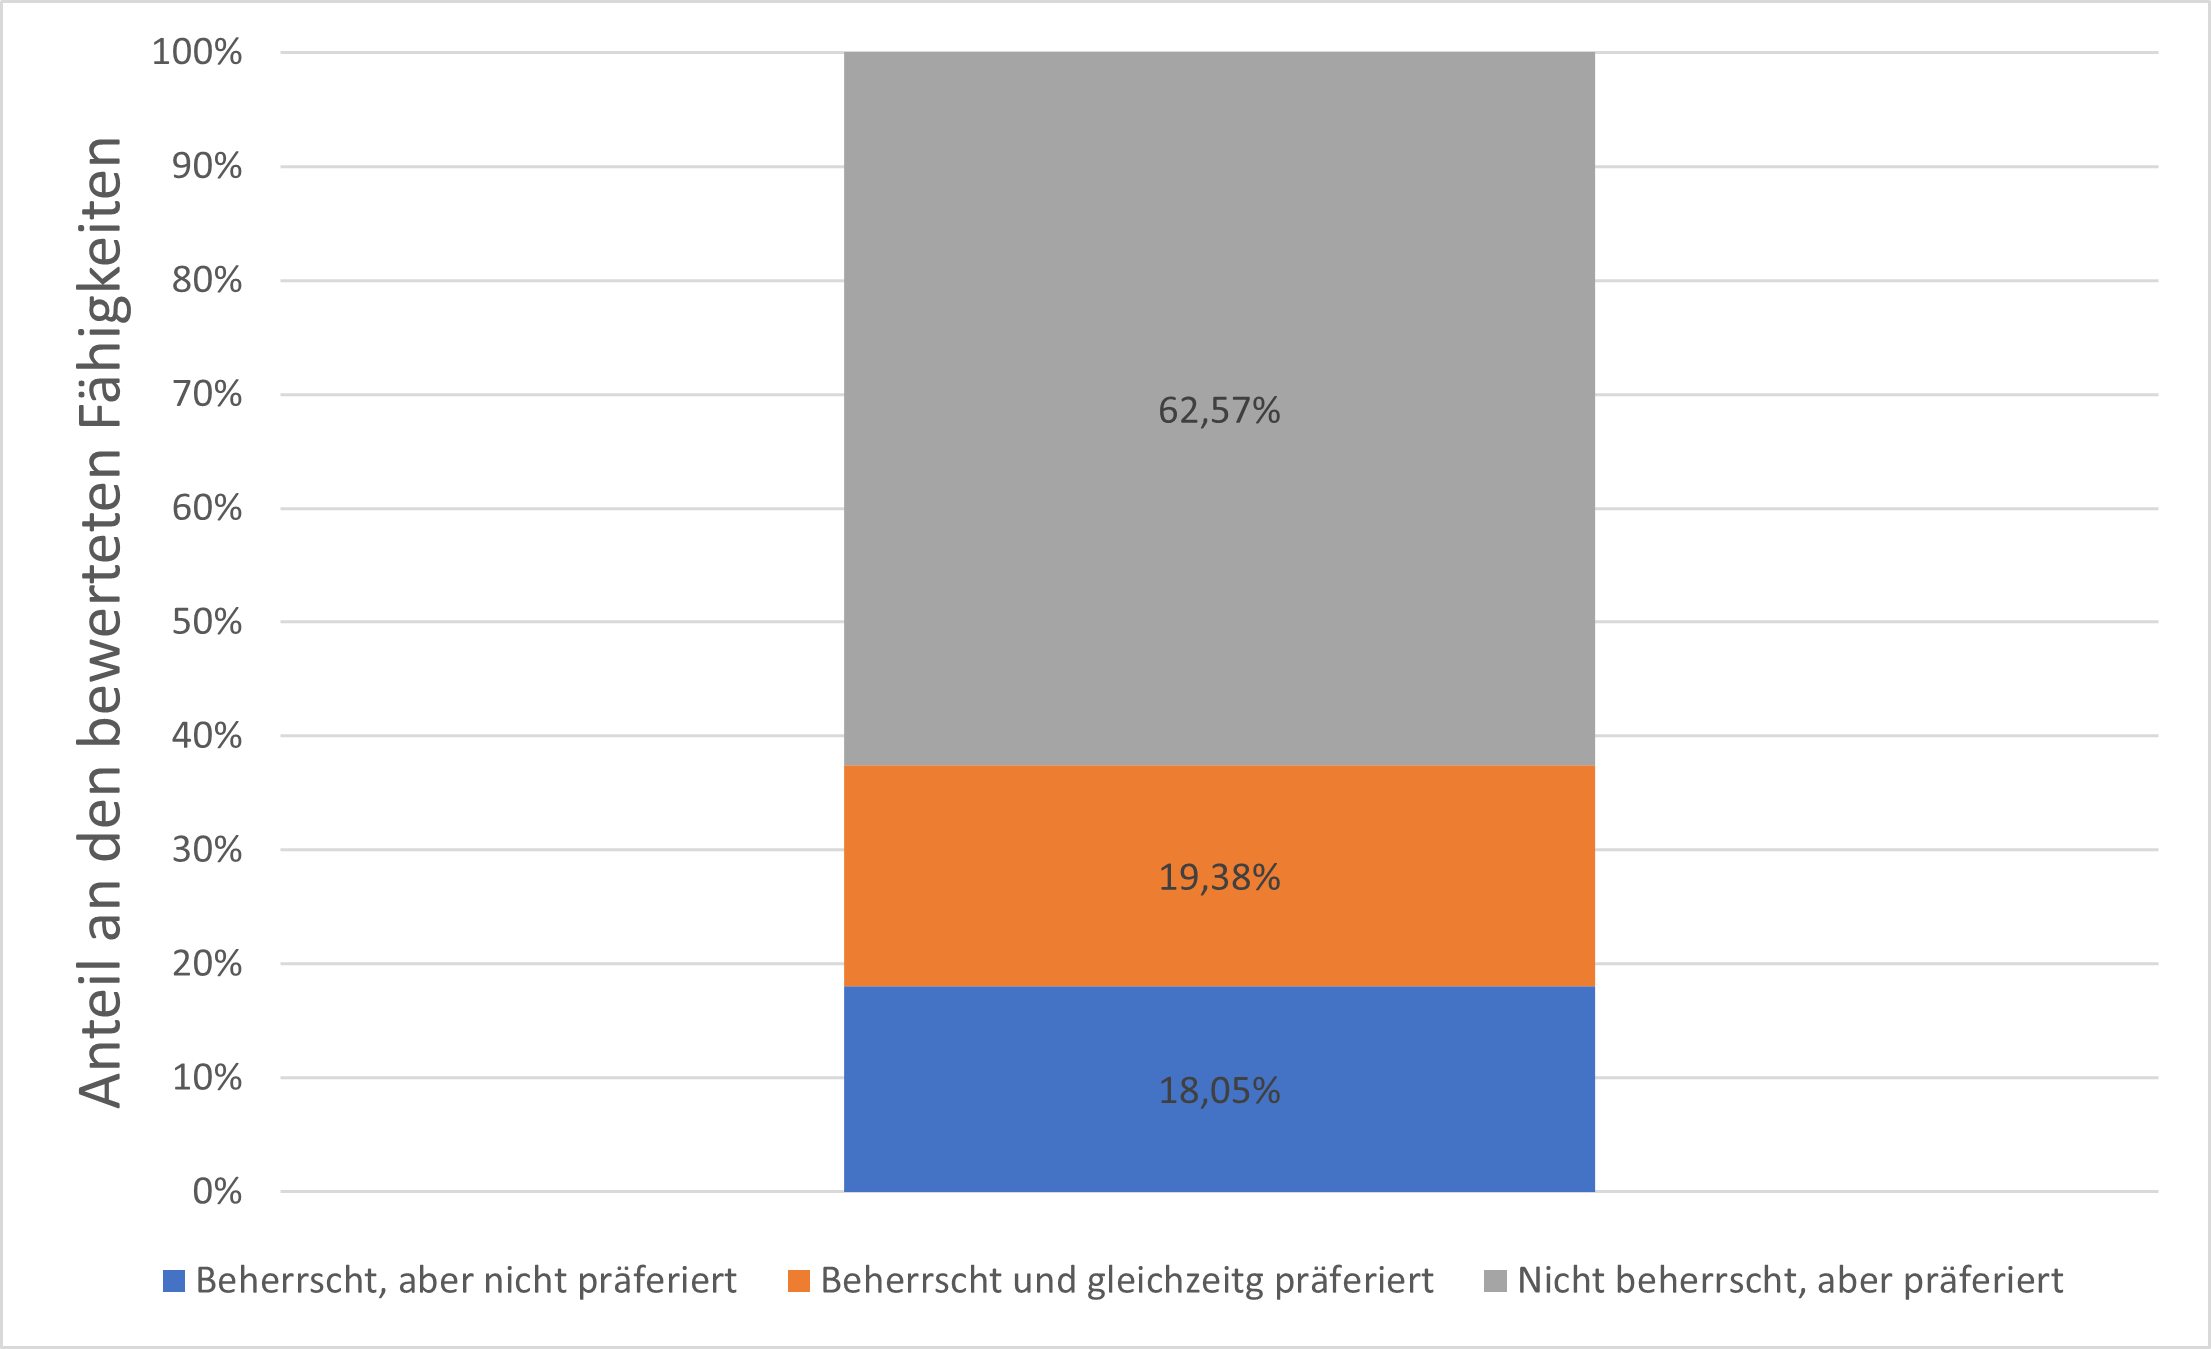
\includegraphics[width=1\textwidth]{gfx/auswertung-anteil-an-faehigkeiten.png}
	\caption{Anteil beherrschter und präferierter Fähigkeiten bei einem durchschnittlichen Mitarbeiter}
	\label{fig:ergebnisse:analyse:abb3}
\end{figure}

In Abbildung \ref{fig:ergebnisse:analyse:abb3} ist zu erkennen, dass ein durchschnittlicher Angestellter etwa 28 bzw. ca. 37.4 Prozent seiner insgesamt beurteilten Kompetenzen gleichzeitig beherrscht (orangene und blaue Farbe). Von diesen Fähigkeiten präferiert er jedoch nur ca. 14.5, also knapp über die Hälfte (orangene Farbe). Demgegenüber stehen ca. 46.7 bzw. etwa 62.6 Prozent an Fähigkeiten, welche der Angestellte zwar präferiert, aber noch nicht beherrscht (graue Farbe).

%Bei Betrachtung der beherrschten Fähigkeiten ist festzustellen, dass kaum Unterschiede zwischen präferierten und nicht gewünschten Kompetenzen ausgemacht werden können. So verfügt die durchschnittliche beherrschte, aber nicht gewünschte Fähigkeit (blaue Farbe in Abbildung \ref{fig:ergebnisse:analyse:abb3}) über eine Bewertung von 2.9 im Intranet. Die durchschnittliche vorhandene und gleichzeitig präferierte Kompetenz (orangene Farbe in Abbildung \ref{fig:ergebnisse:analyse:abb3}) verfügt über eine Bewertung von 3.1. Wie in Abbildung \ref{fig:ergebnisse:analyse:abb4} zu erkennen, sind auch bei Betrachtung der Fähigkeiten auf ihren jeweiligen Kompetenzniveaus kaum Differenzen auszumachen.
%\begin{figure}[h]
%	\centering
%	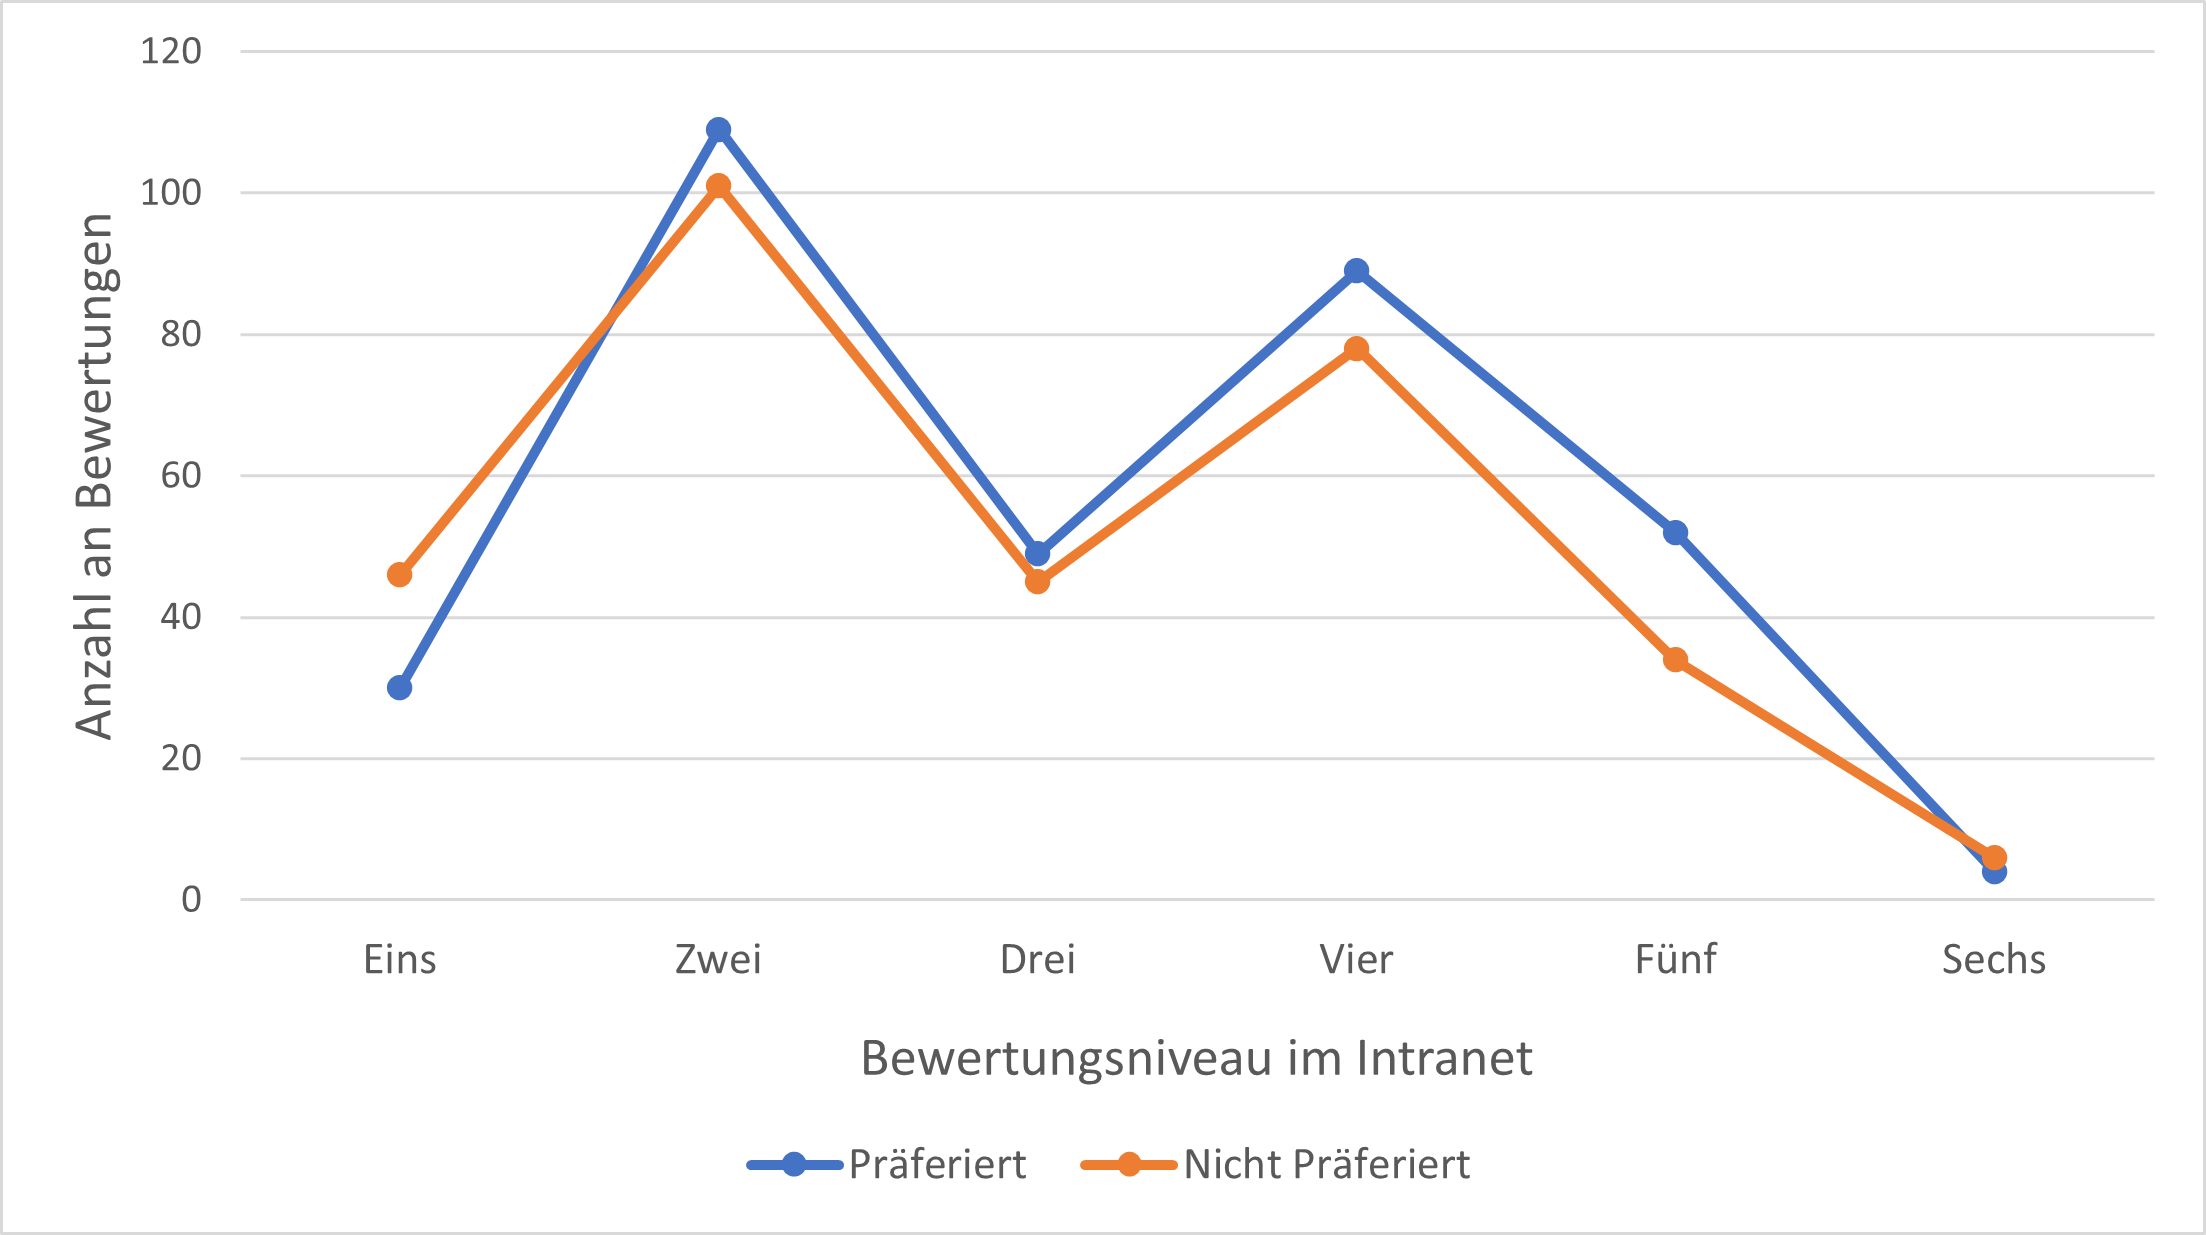
\includegraphics[width=0.8\textwidth]{gfx/bewertungen-je-bewertungsniveau.png}
%	\caption{Anzahl beherrschter und präferierter Fähigkeiten je Bewertungsniveau}
%	\label{fig:ergebnisse:analyse:abb4}
%\end{figure}
%Bei Analyse der präferierten Fähigkeiten (graue Farbe in Abbildung \ref{fig:ergebnisse:analyse:abb3}) ist zu beobachten, dass es sich bei den meist gewünschten Kompetenzen hauptsächlich um moderne Produkte aus dem Web- und Cloud-Umfeld handelt. So zählen neben Git und Java beispielsweise Kotlin, Kubernetes, Docker, Spring Boot und AWS zu den meist präferierten Fähigkeiten.

\subsection{Gesuchte und vorhandene Fähigkeiten und Präferenzen}
\label{ch:ergebnisse:umfrageMitarbeiter:projekte}
Zur Beantwortung der Forschungsfrage wurden im Rahmen der vorliegenden Master-Thesis fünf beispielhafte Projektpositionen definiert und in Kapitel \ref{ch:methodik:evaluation} vorgestellt. Abbildung \ref{fig:ergebnisse:analyse:abb5} zeigt für jede dieser Projektpositionen, wie viele der befragten Mitarbeiter im Durchschnitt die gesuchten Fähigkeiten beherrschen bzw. präferieren.

\begin{figure}[h]
	\centering
	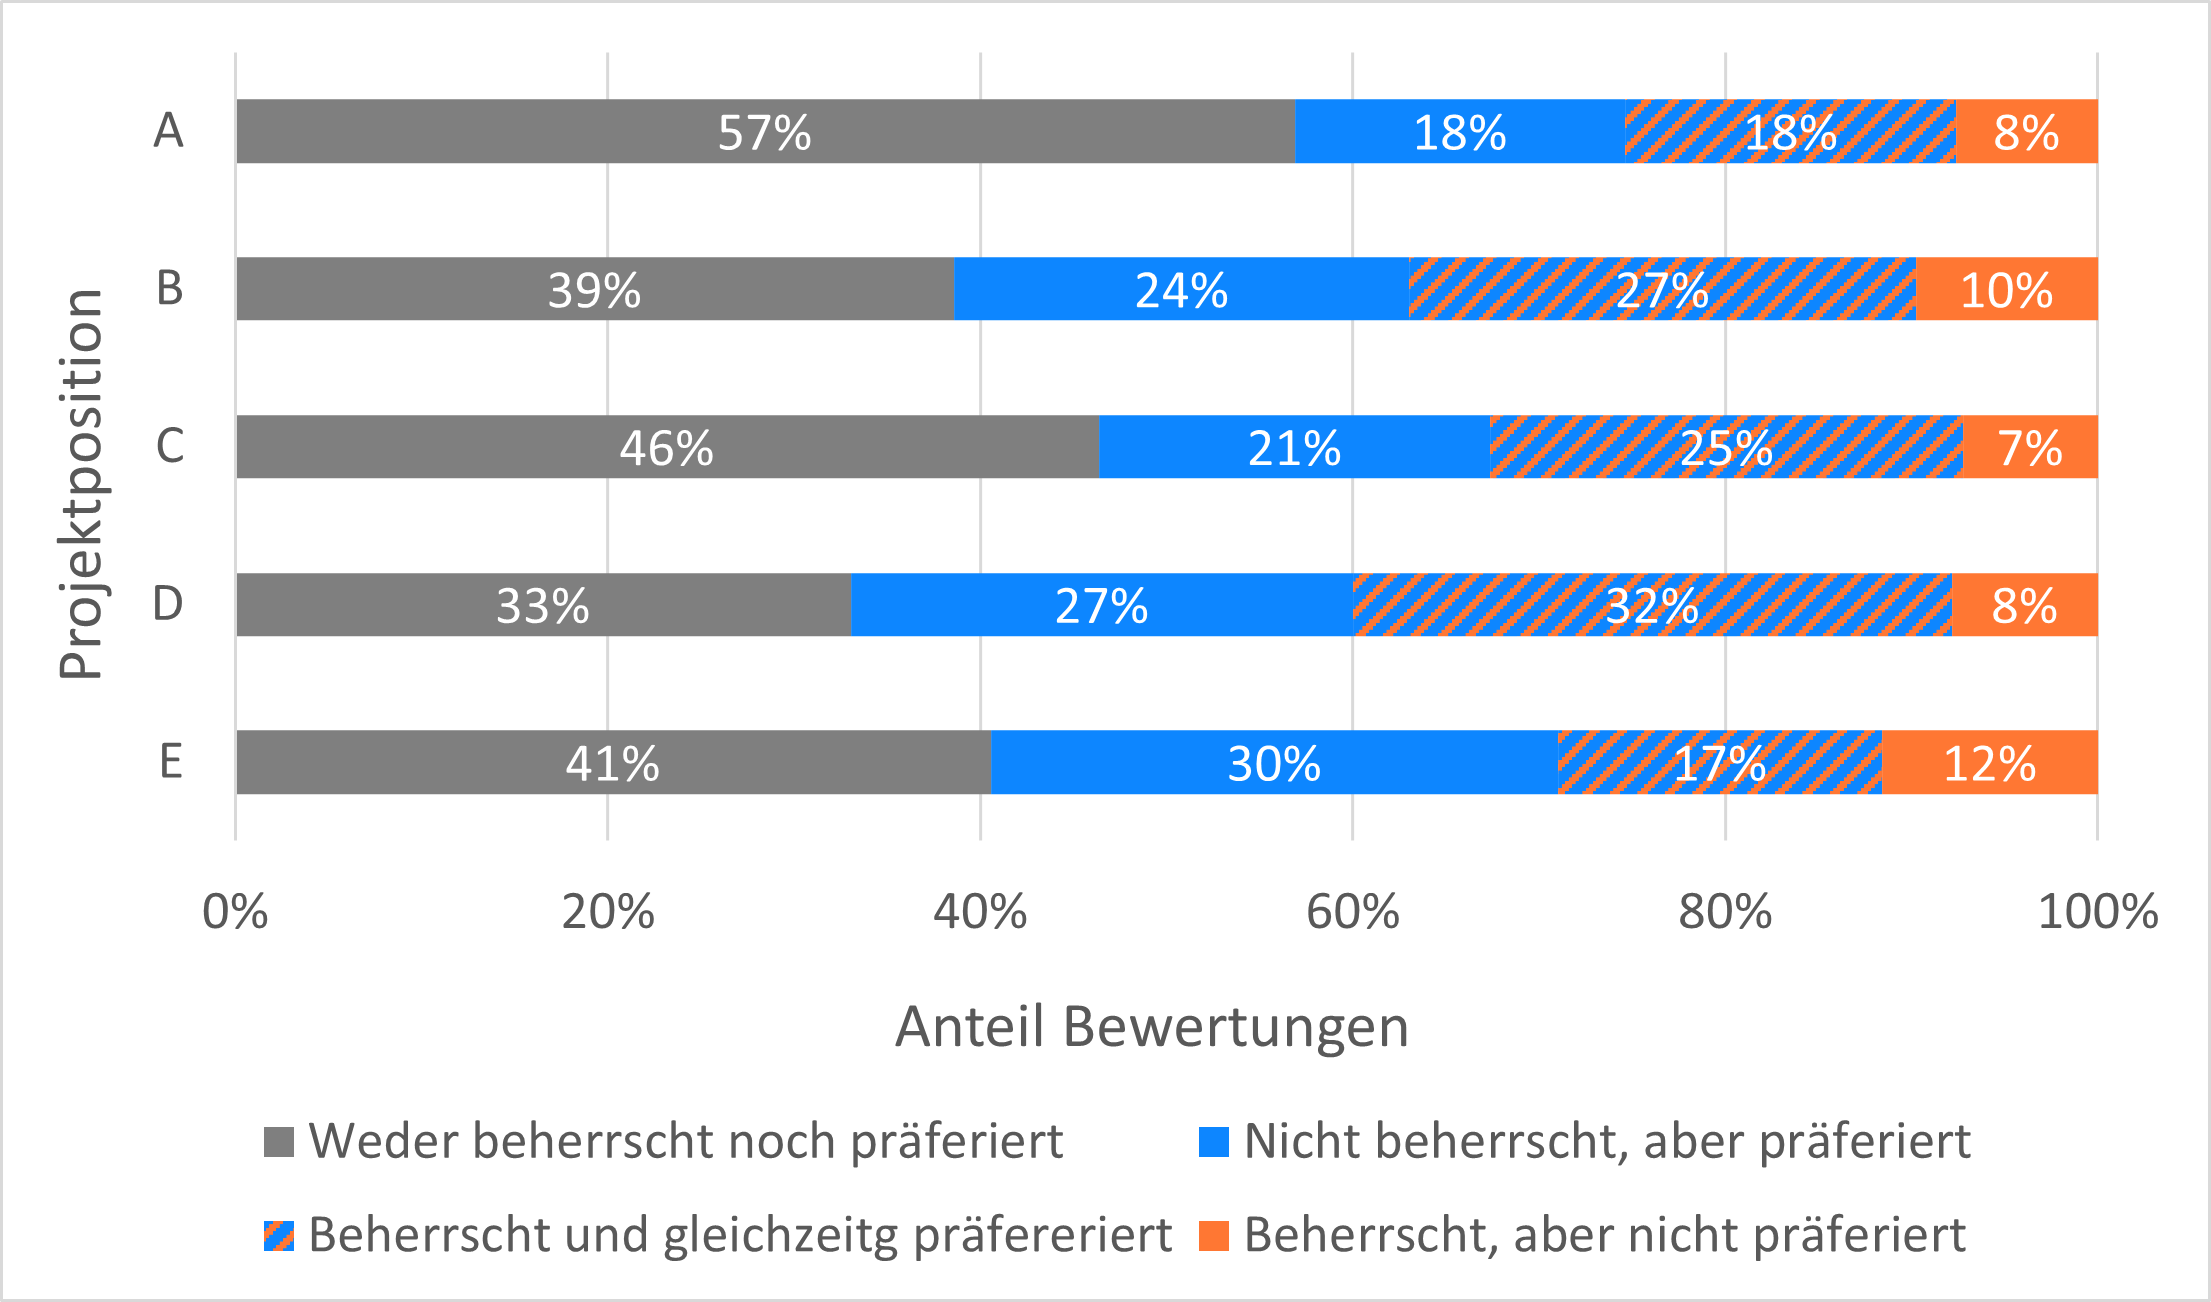
\includegraphics[width=1\textwidth]{gfx/anteil-bewertungen-je-projektposition.png}
	\caption{Anteil an Mitarbeitern, welche die in den Beispielprojektpositionen gesuchten Fähigkeiten im Durchschnitt beherrschen bzw. präferieren}
	\label{fig:ergebnisse:analyse:abb5}
\end{figure}

In Abbildung \ref{fig:ergebnisse:analyse:abb5} ist zu erkennen, dass durchschnittlich 33 Prozent aller Mitarbeiter bereits über die für die Projektpositionen benötigten Fähigkeiten verfügen. Dementsprechend beherrschen 67 Prozent aller Mitarbeiter die durchschnittlich gesuchte Kompetenz noch nicht. Es ist ebenfalls du beobachten, dass 60 Prozent aller Angestellten, welche die durchschnittlich gesuchte Kompetenz beherrschen, diese gleichzeitig präferieren. Auch ist zu erkennen, dass die Anteile an Mitarbeitern, welche die durchschnittlich gesuchte Fähigkeit beherrschen und gleichzeitig präferieren und Angestellten, welche die im Durchschnitt benötigte Kompetenz noch nicht beherrschen und dennoch präferieren mit je 24 Prozent gleich groß sind.

Bei Betrachtung jeder einzelnen in den Beispielprojektpositionen gesuchten Fähigkeit ergibt sich die Darstellung aus Abbildung \ref{fig:ergebnisse:analyse:abb6}.

\begin{figure}[h]
	\centering
	
	\subfloat[Projektposition A]{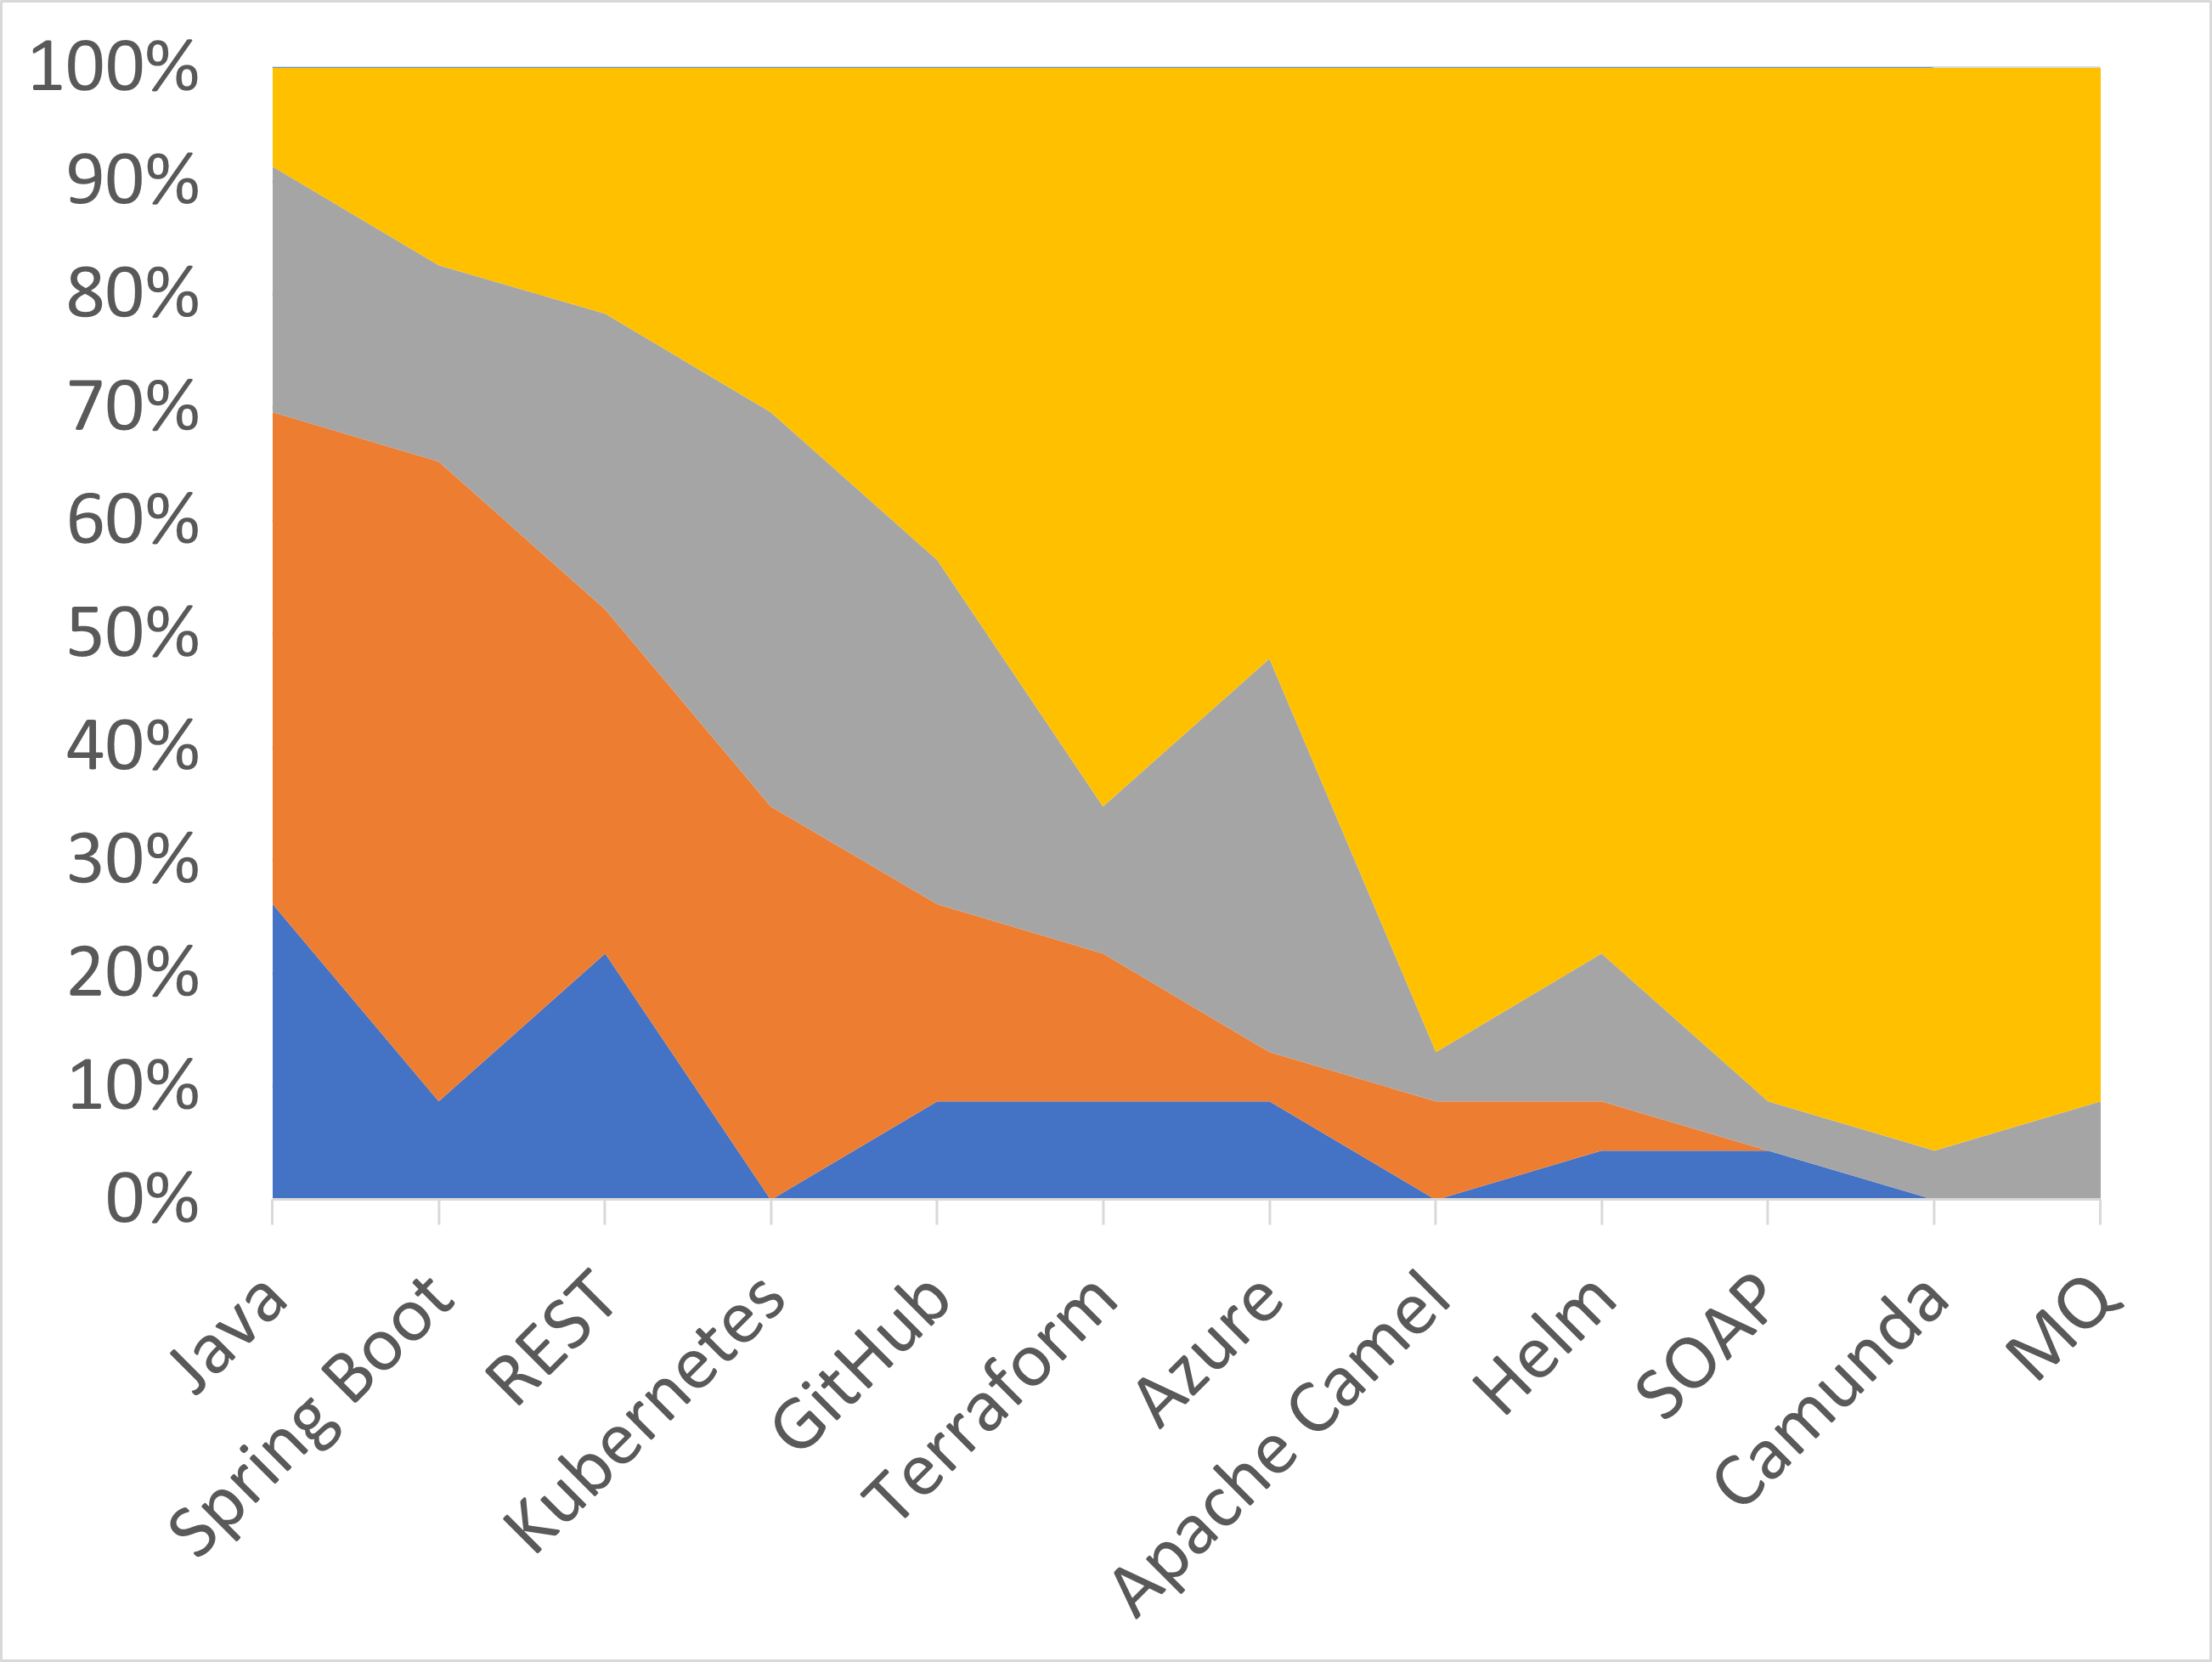
\includegraphics[width = 0.4\textwidth]{gfx/projekt-detail-a.png}}
	\subfloat[Projektposition B]{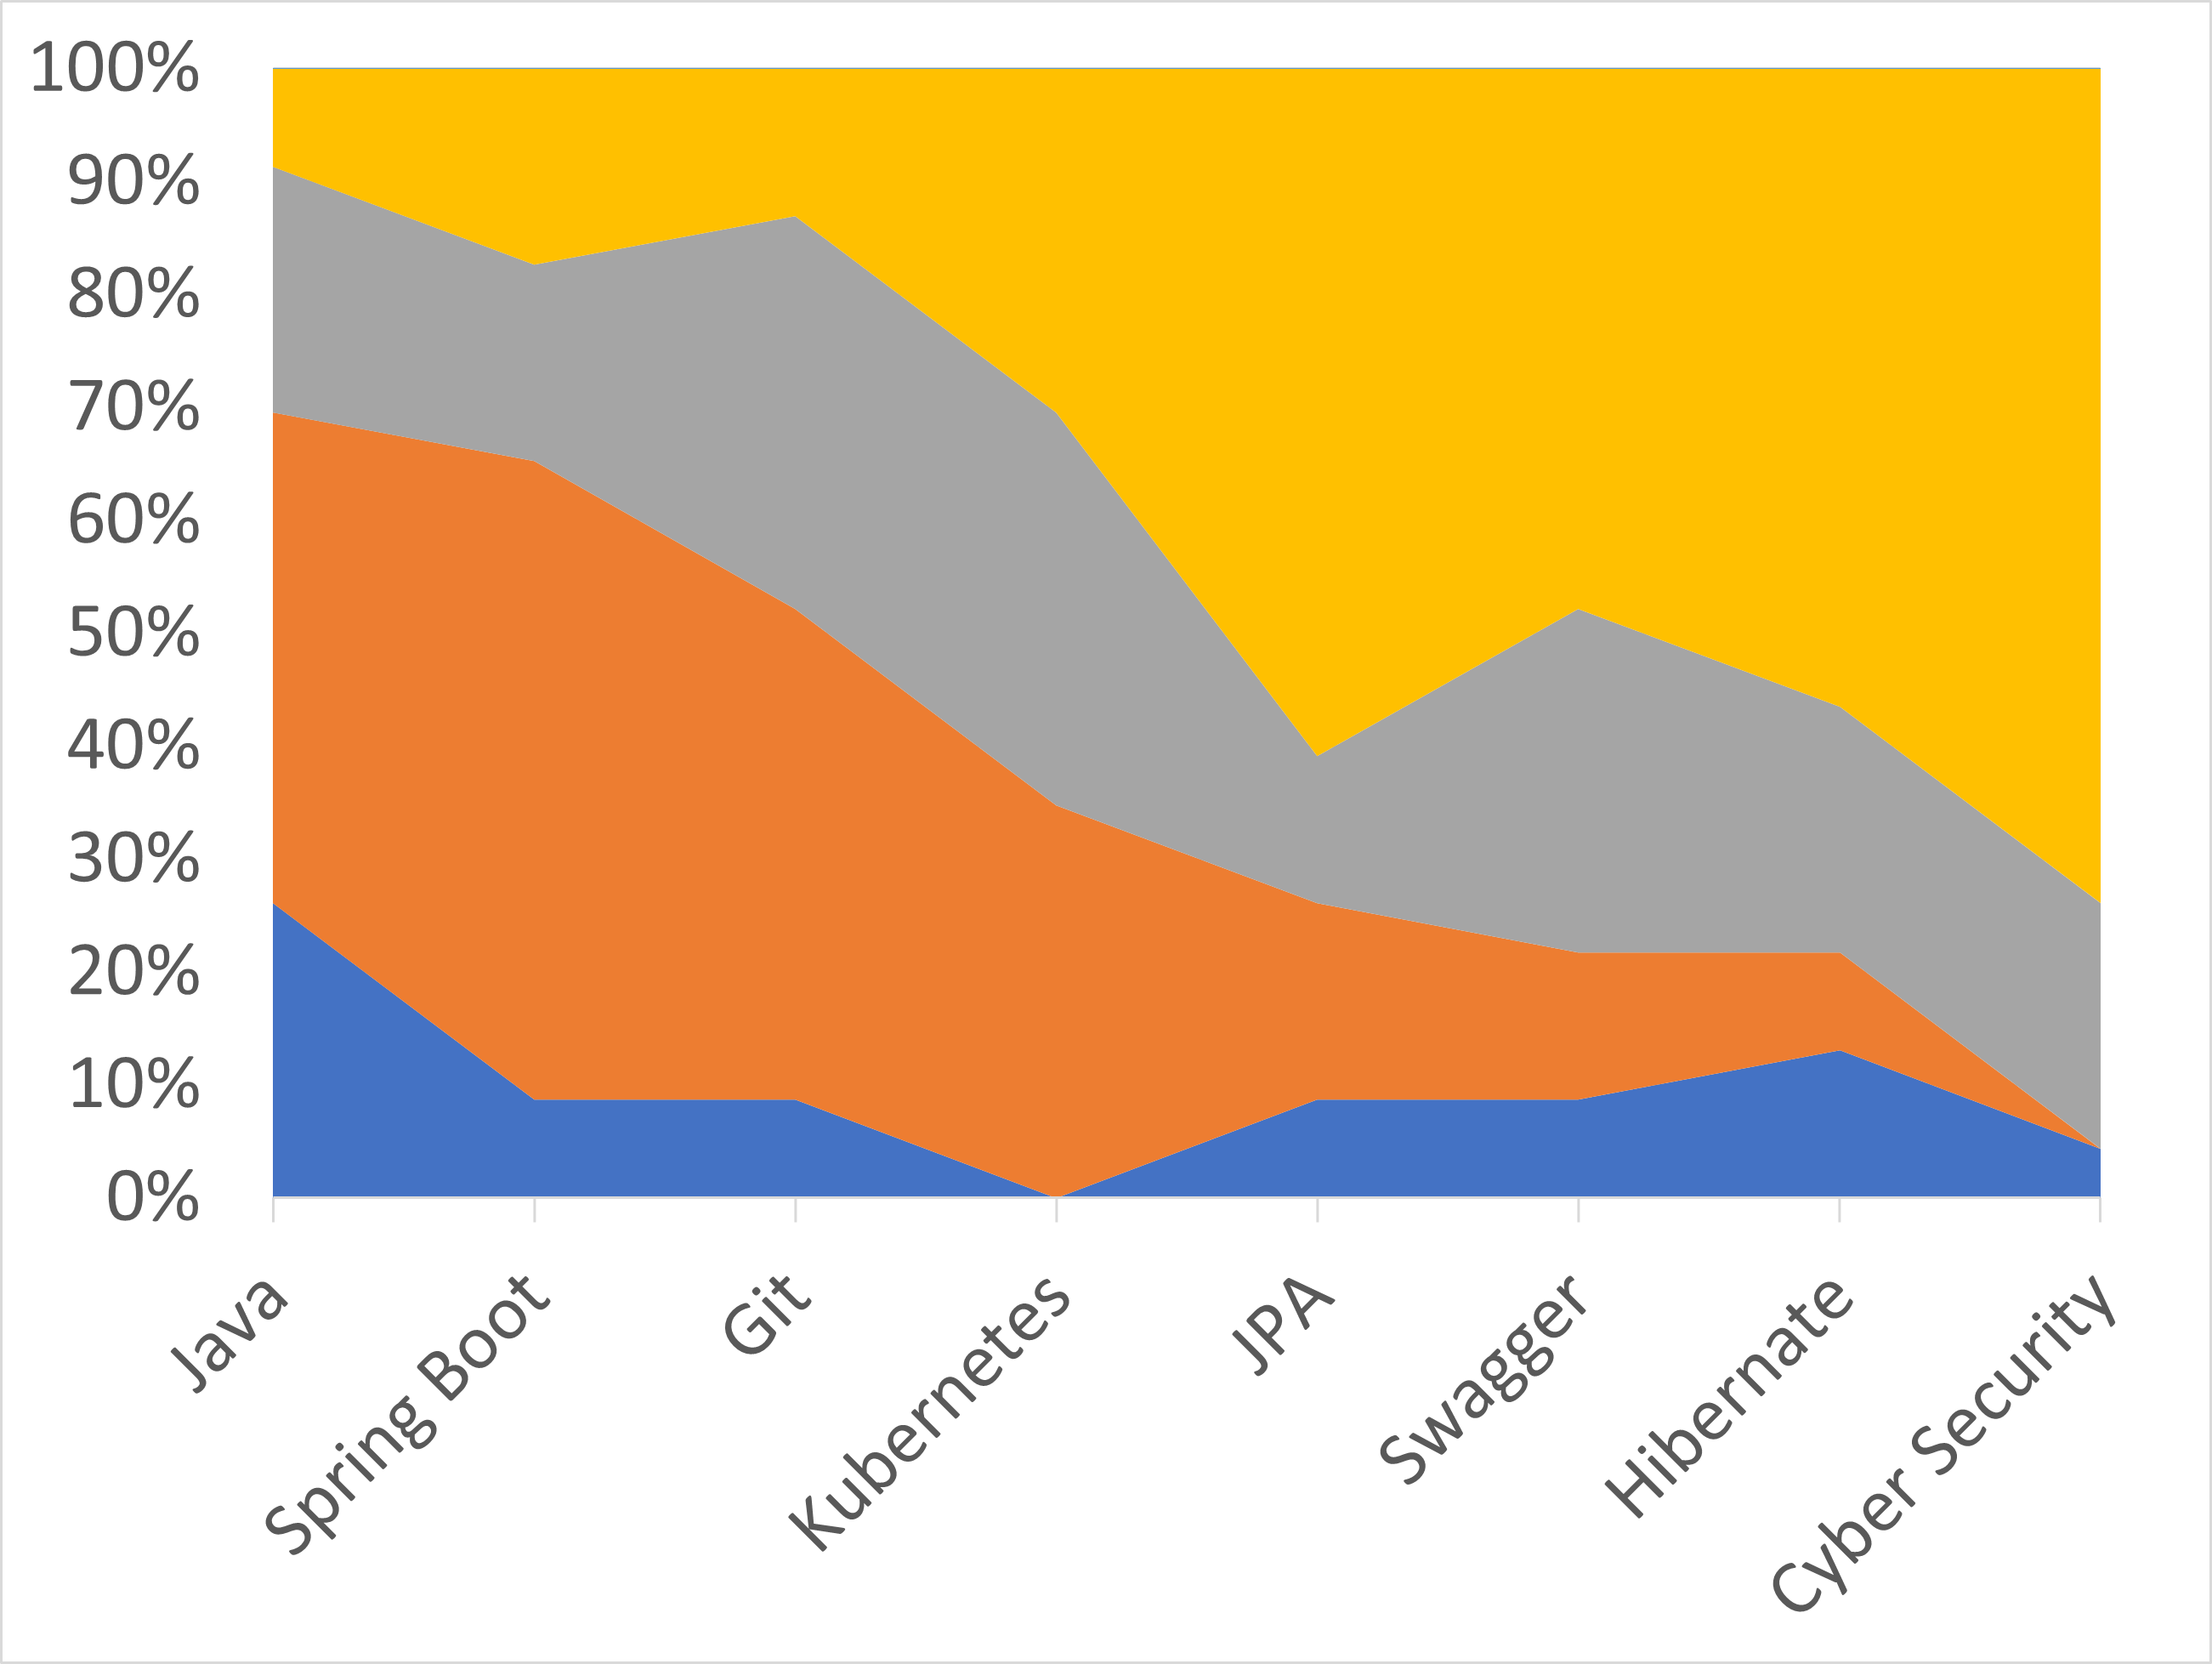
\includegraphics[width = 0.4\textwidth]{gfx/projekt-detail-b.png}}
	\newline	
	\subfloat[Projektposition C]{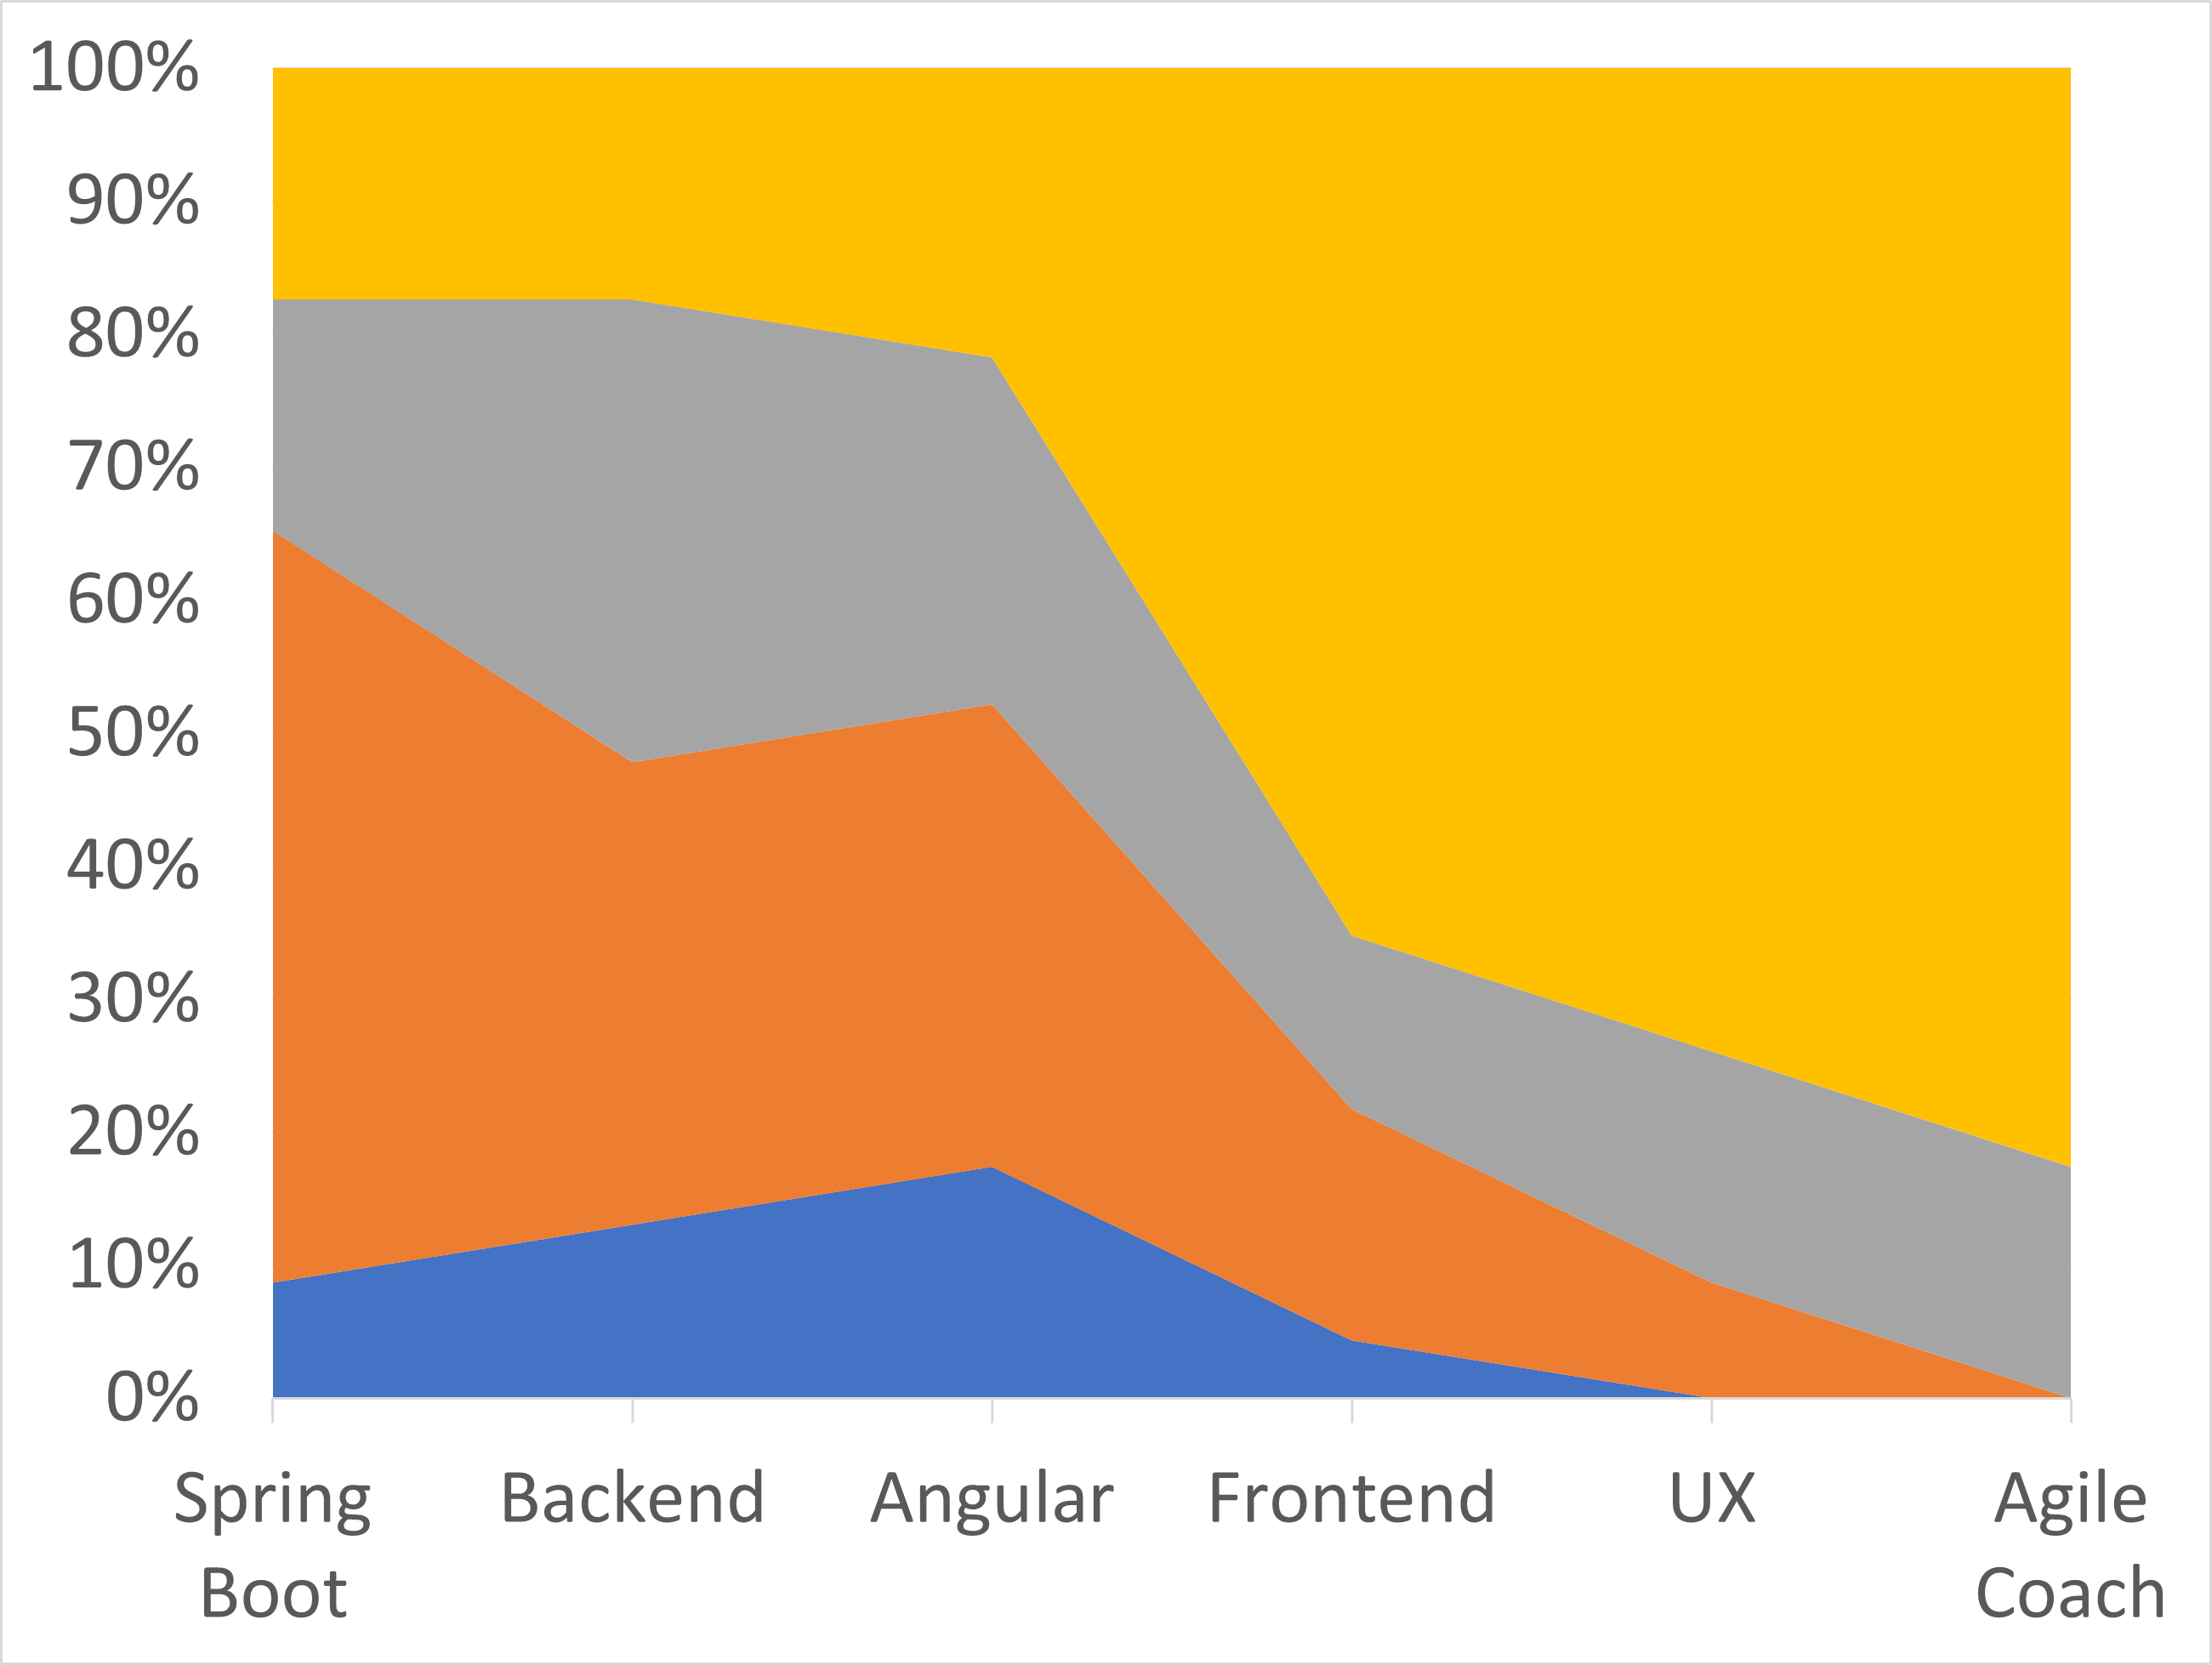
\includegraphics[width = 0.4\textwidth]{gfx/projekt-detail-c.png}}
	\subfloat[Projektposition D]{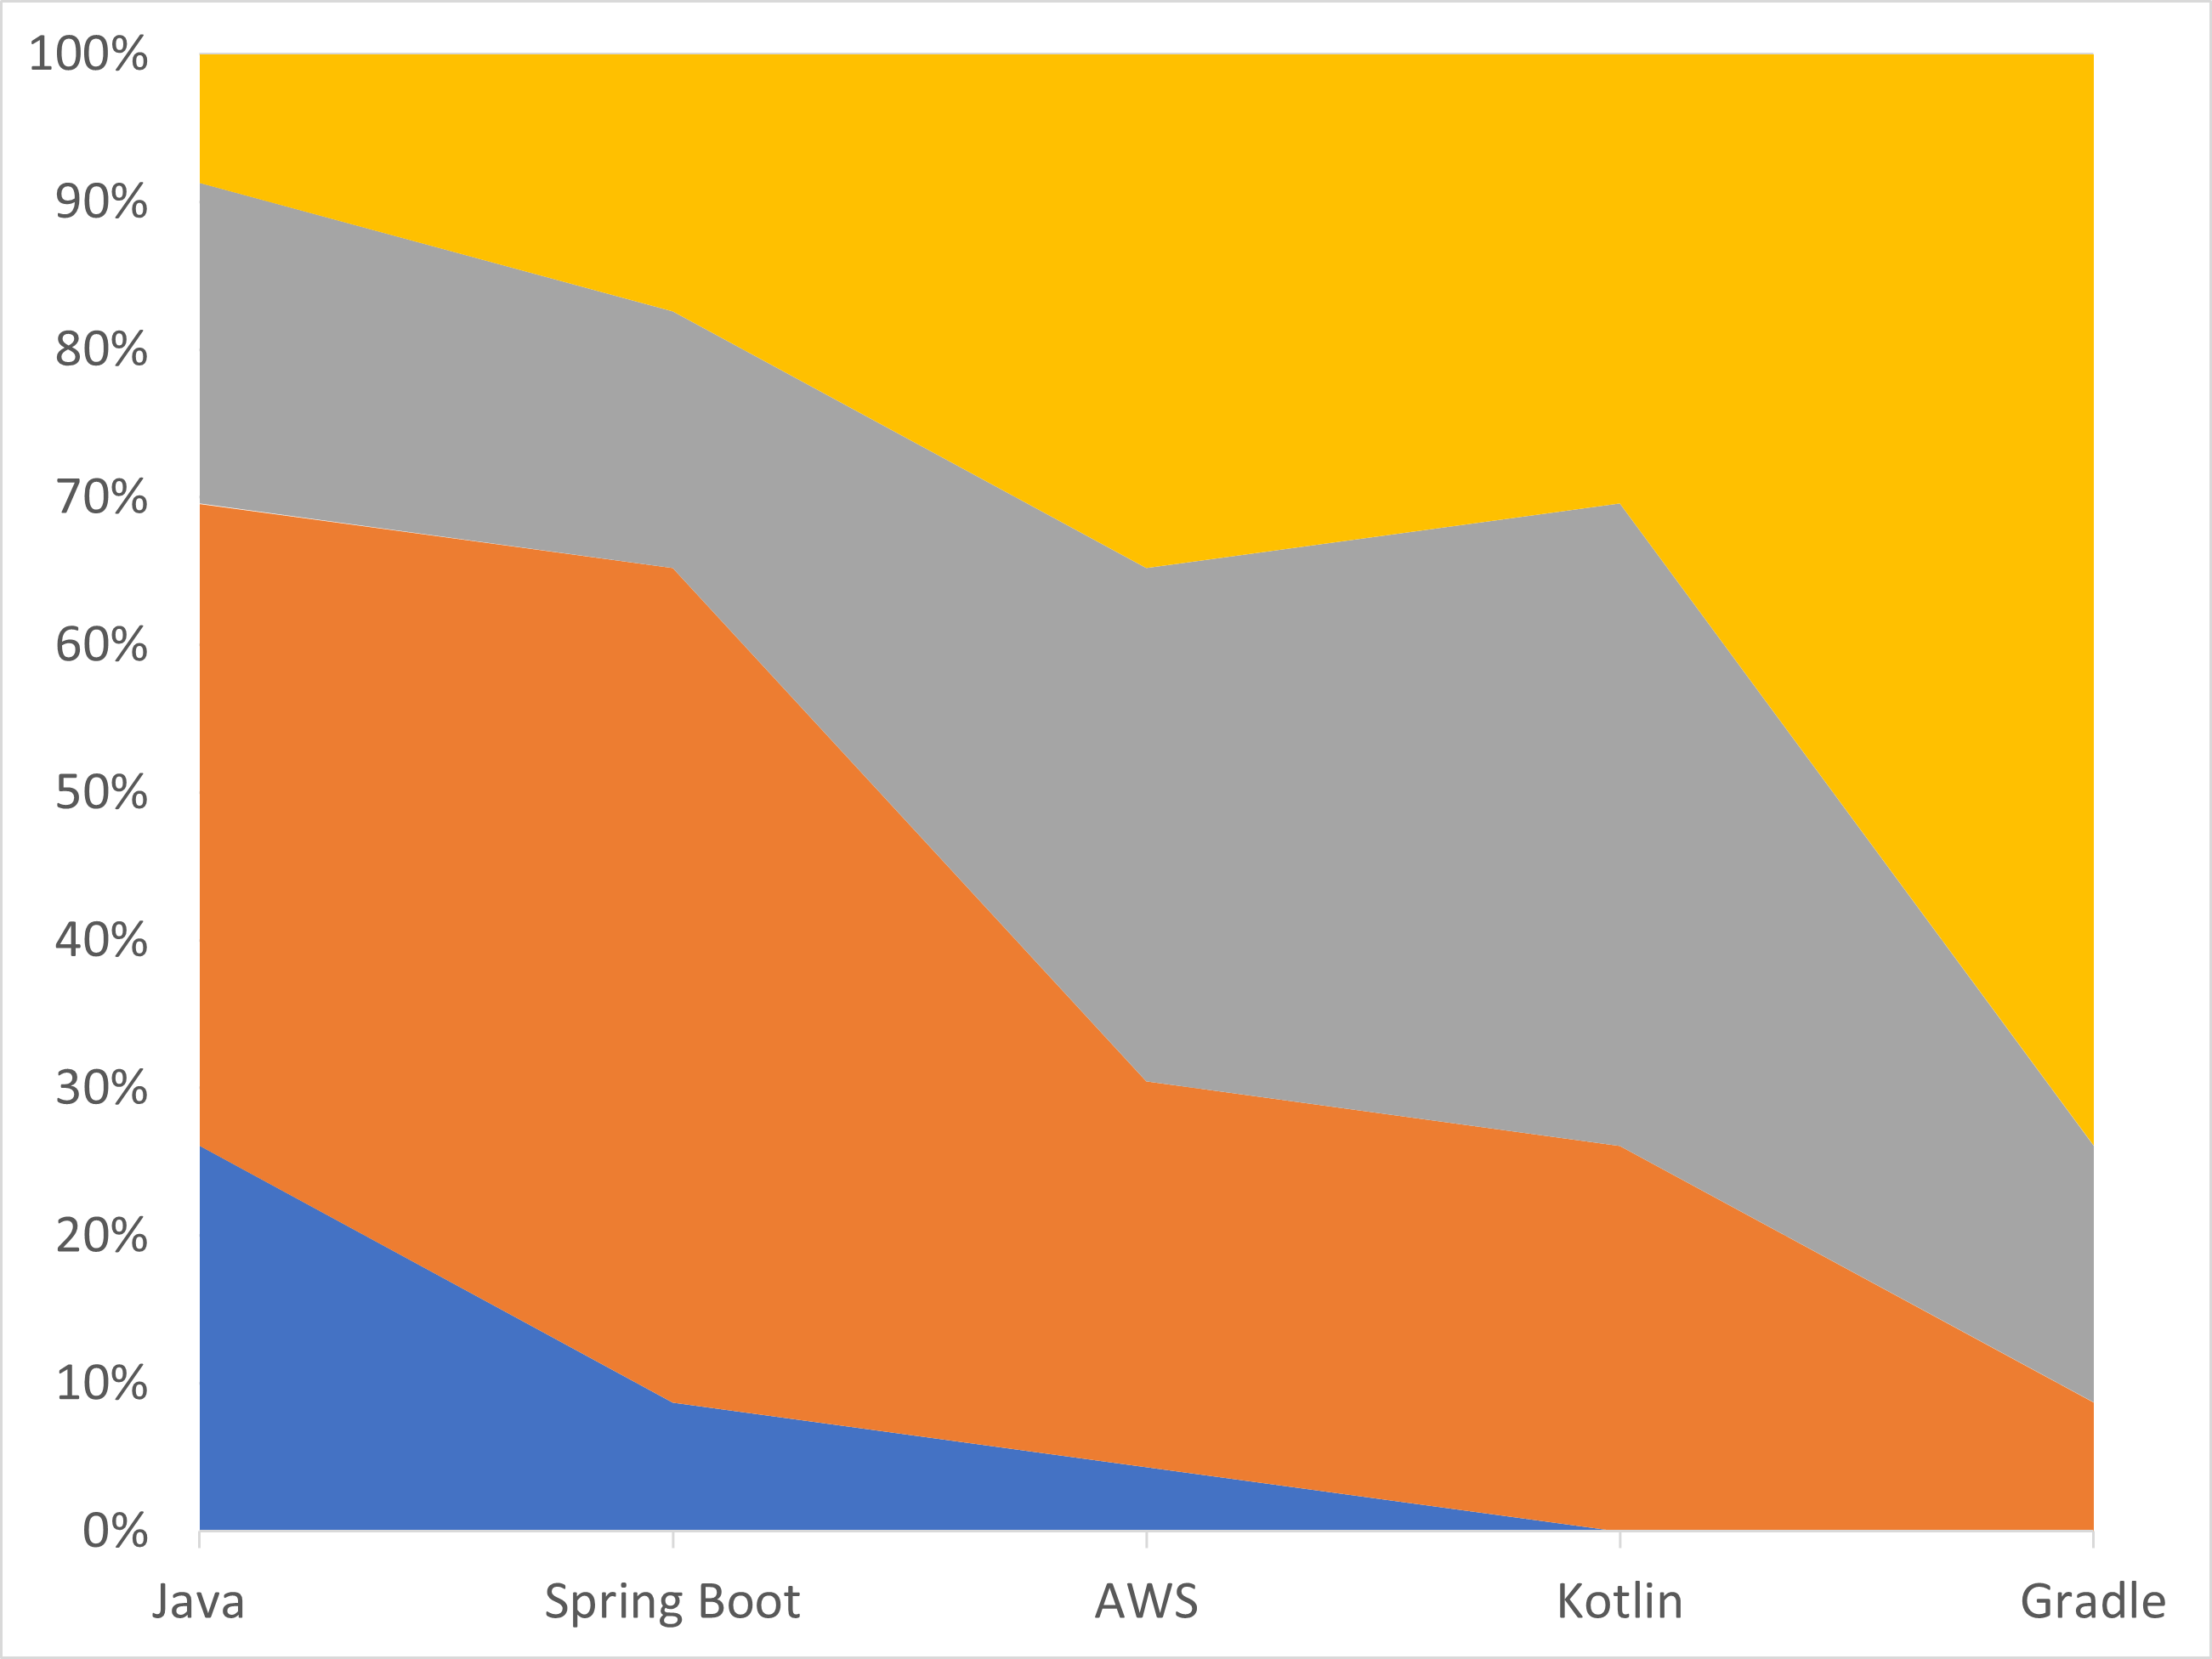
\includegraphics[width = 0.4\textwidth]{gfx/projekt-detail-d.png}}
	\newline
	\subfloat[Projektposition E]{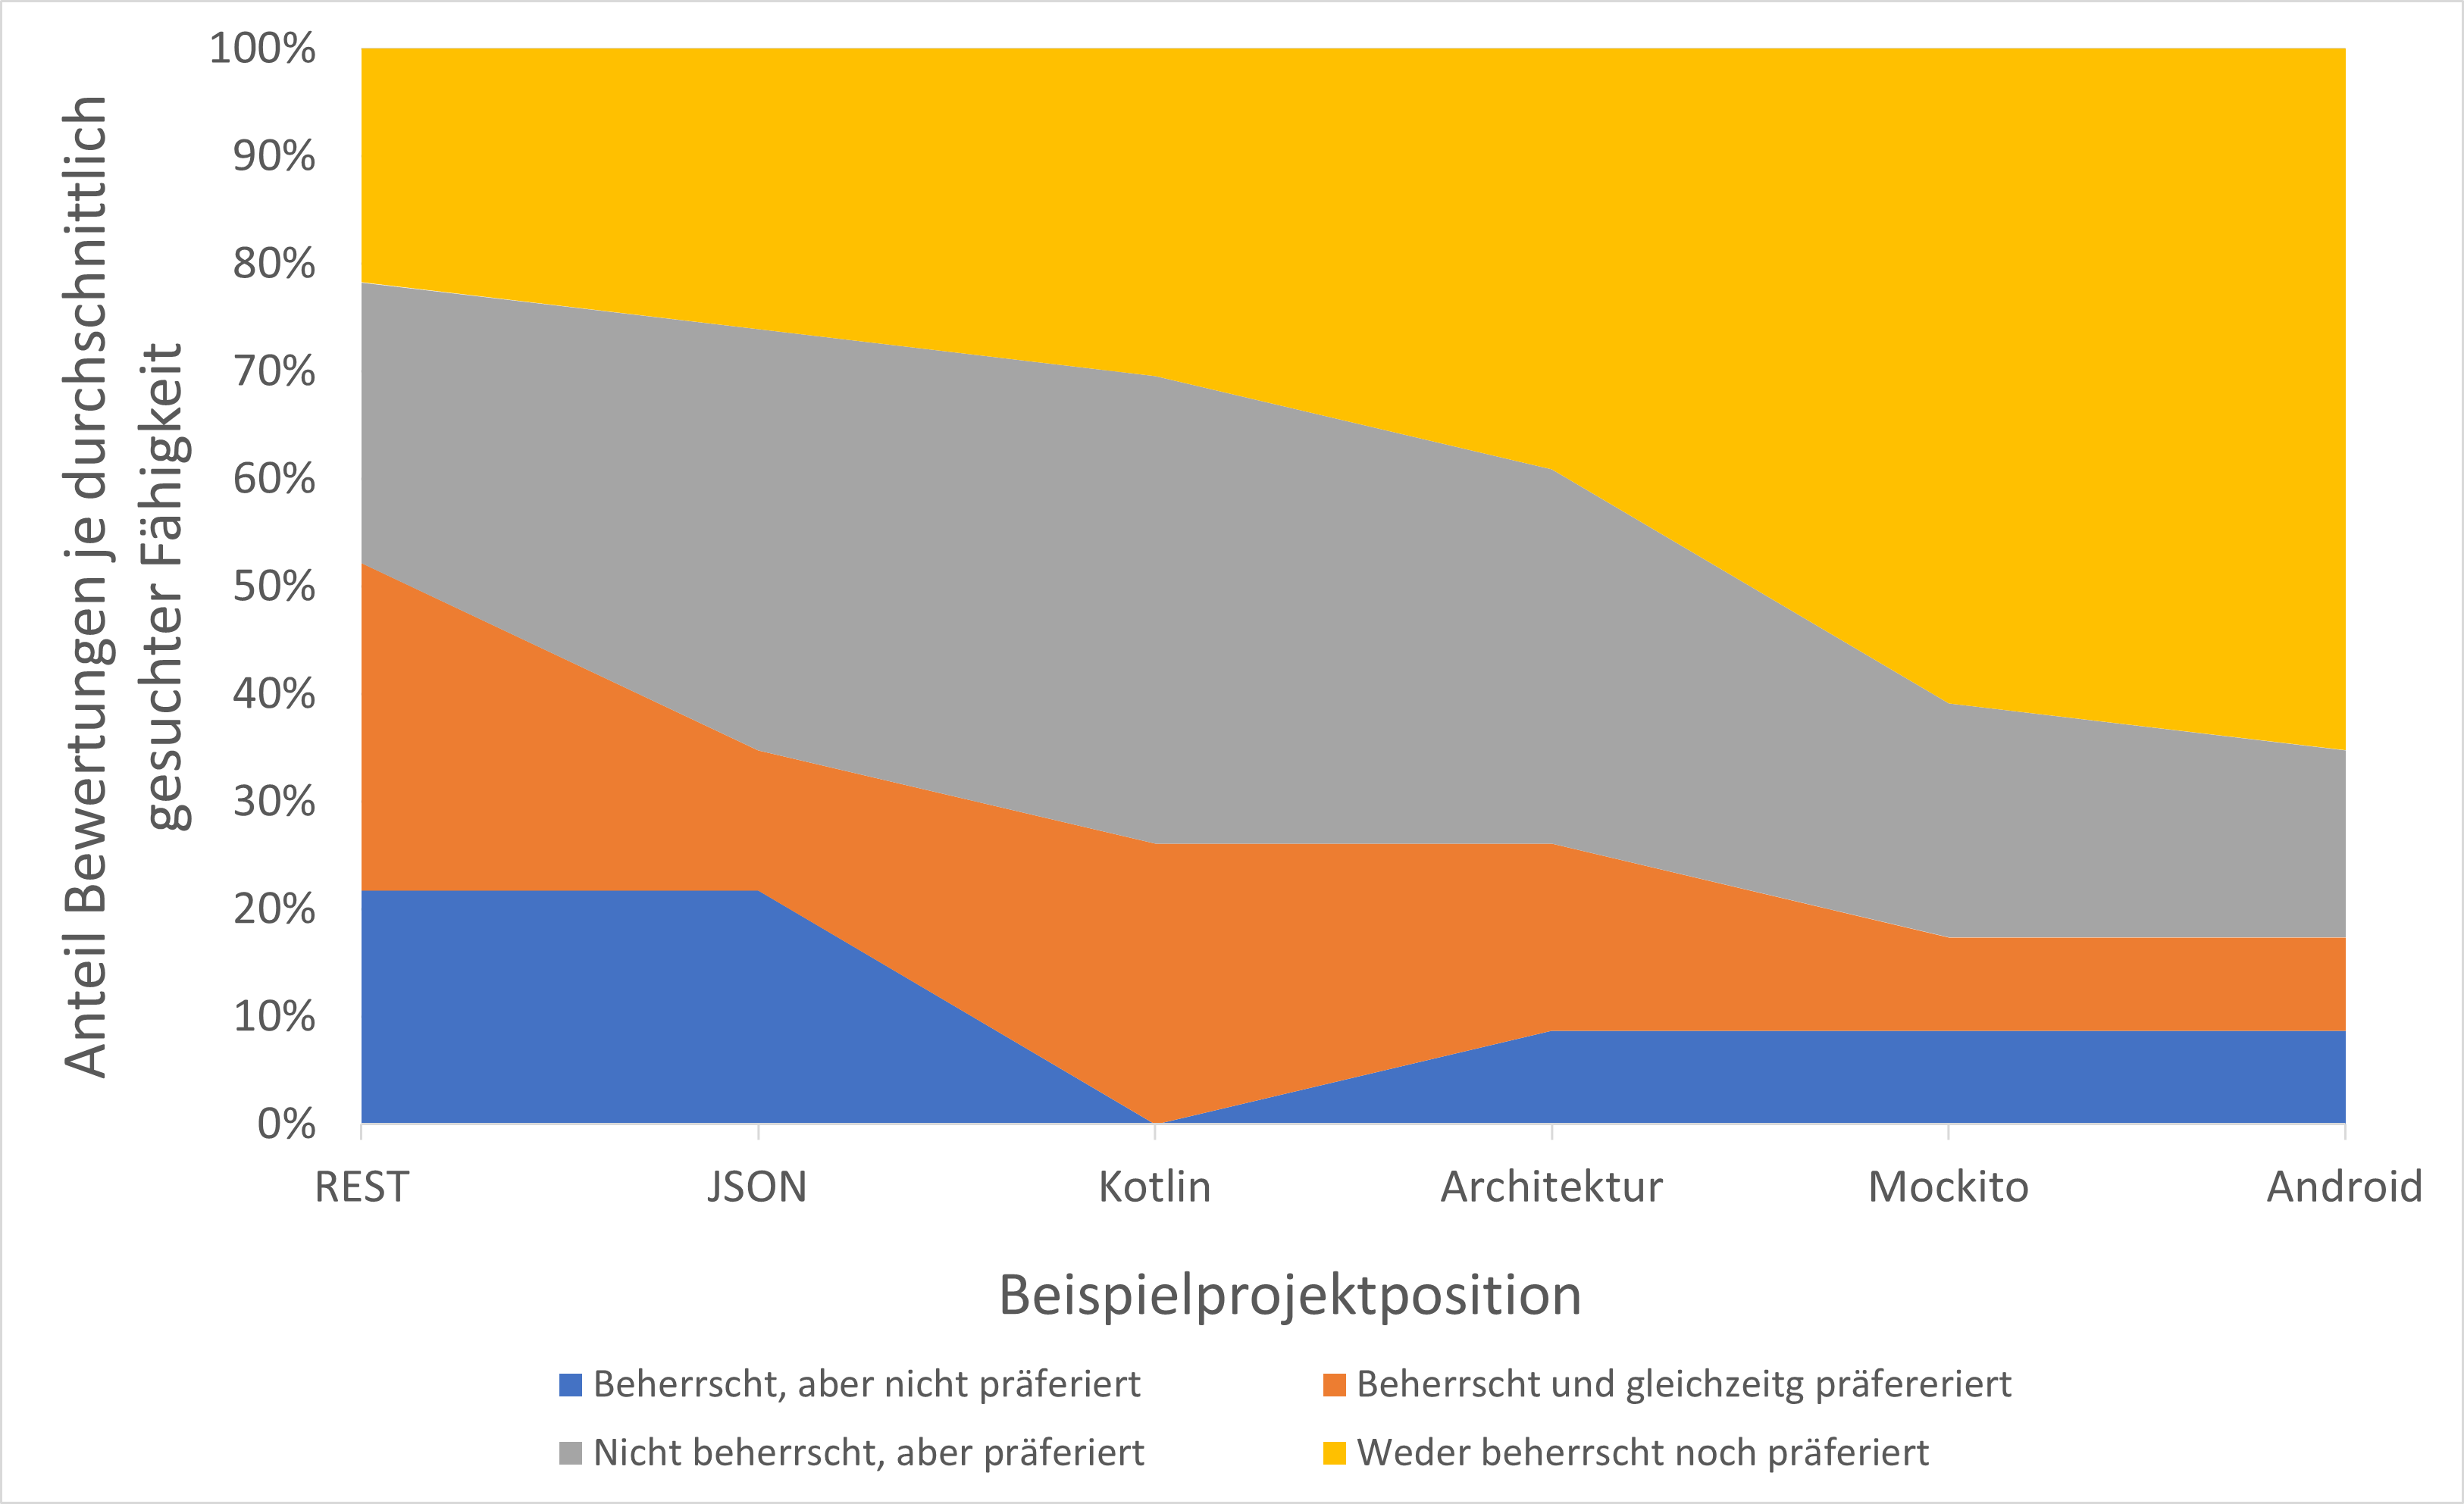
\includegraphics[width = 0.4\textwidth]{gfx/projekt-detail-e.png}}
	\subfloat[Legende]{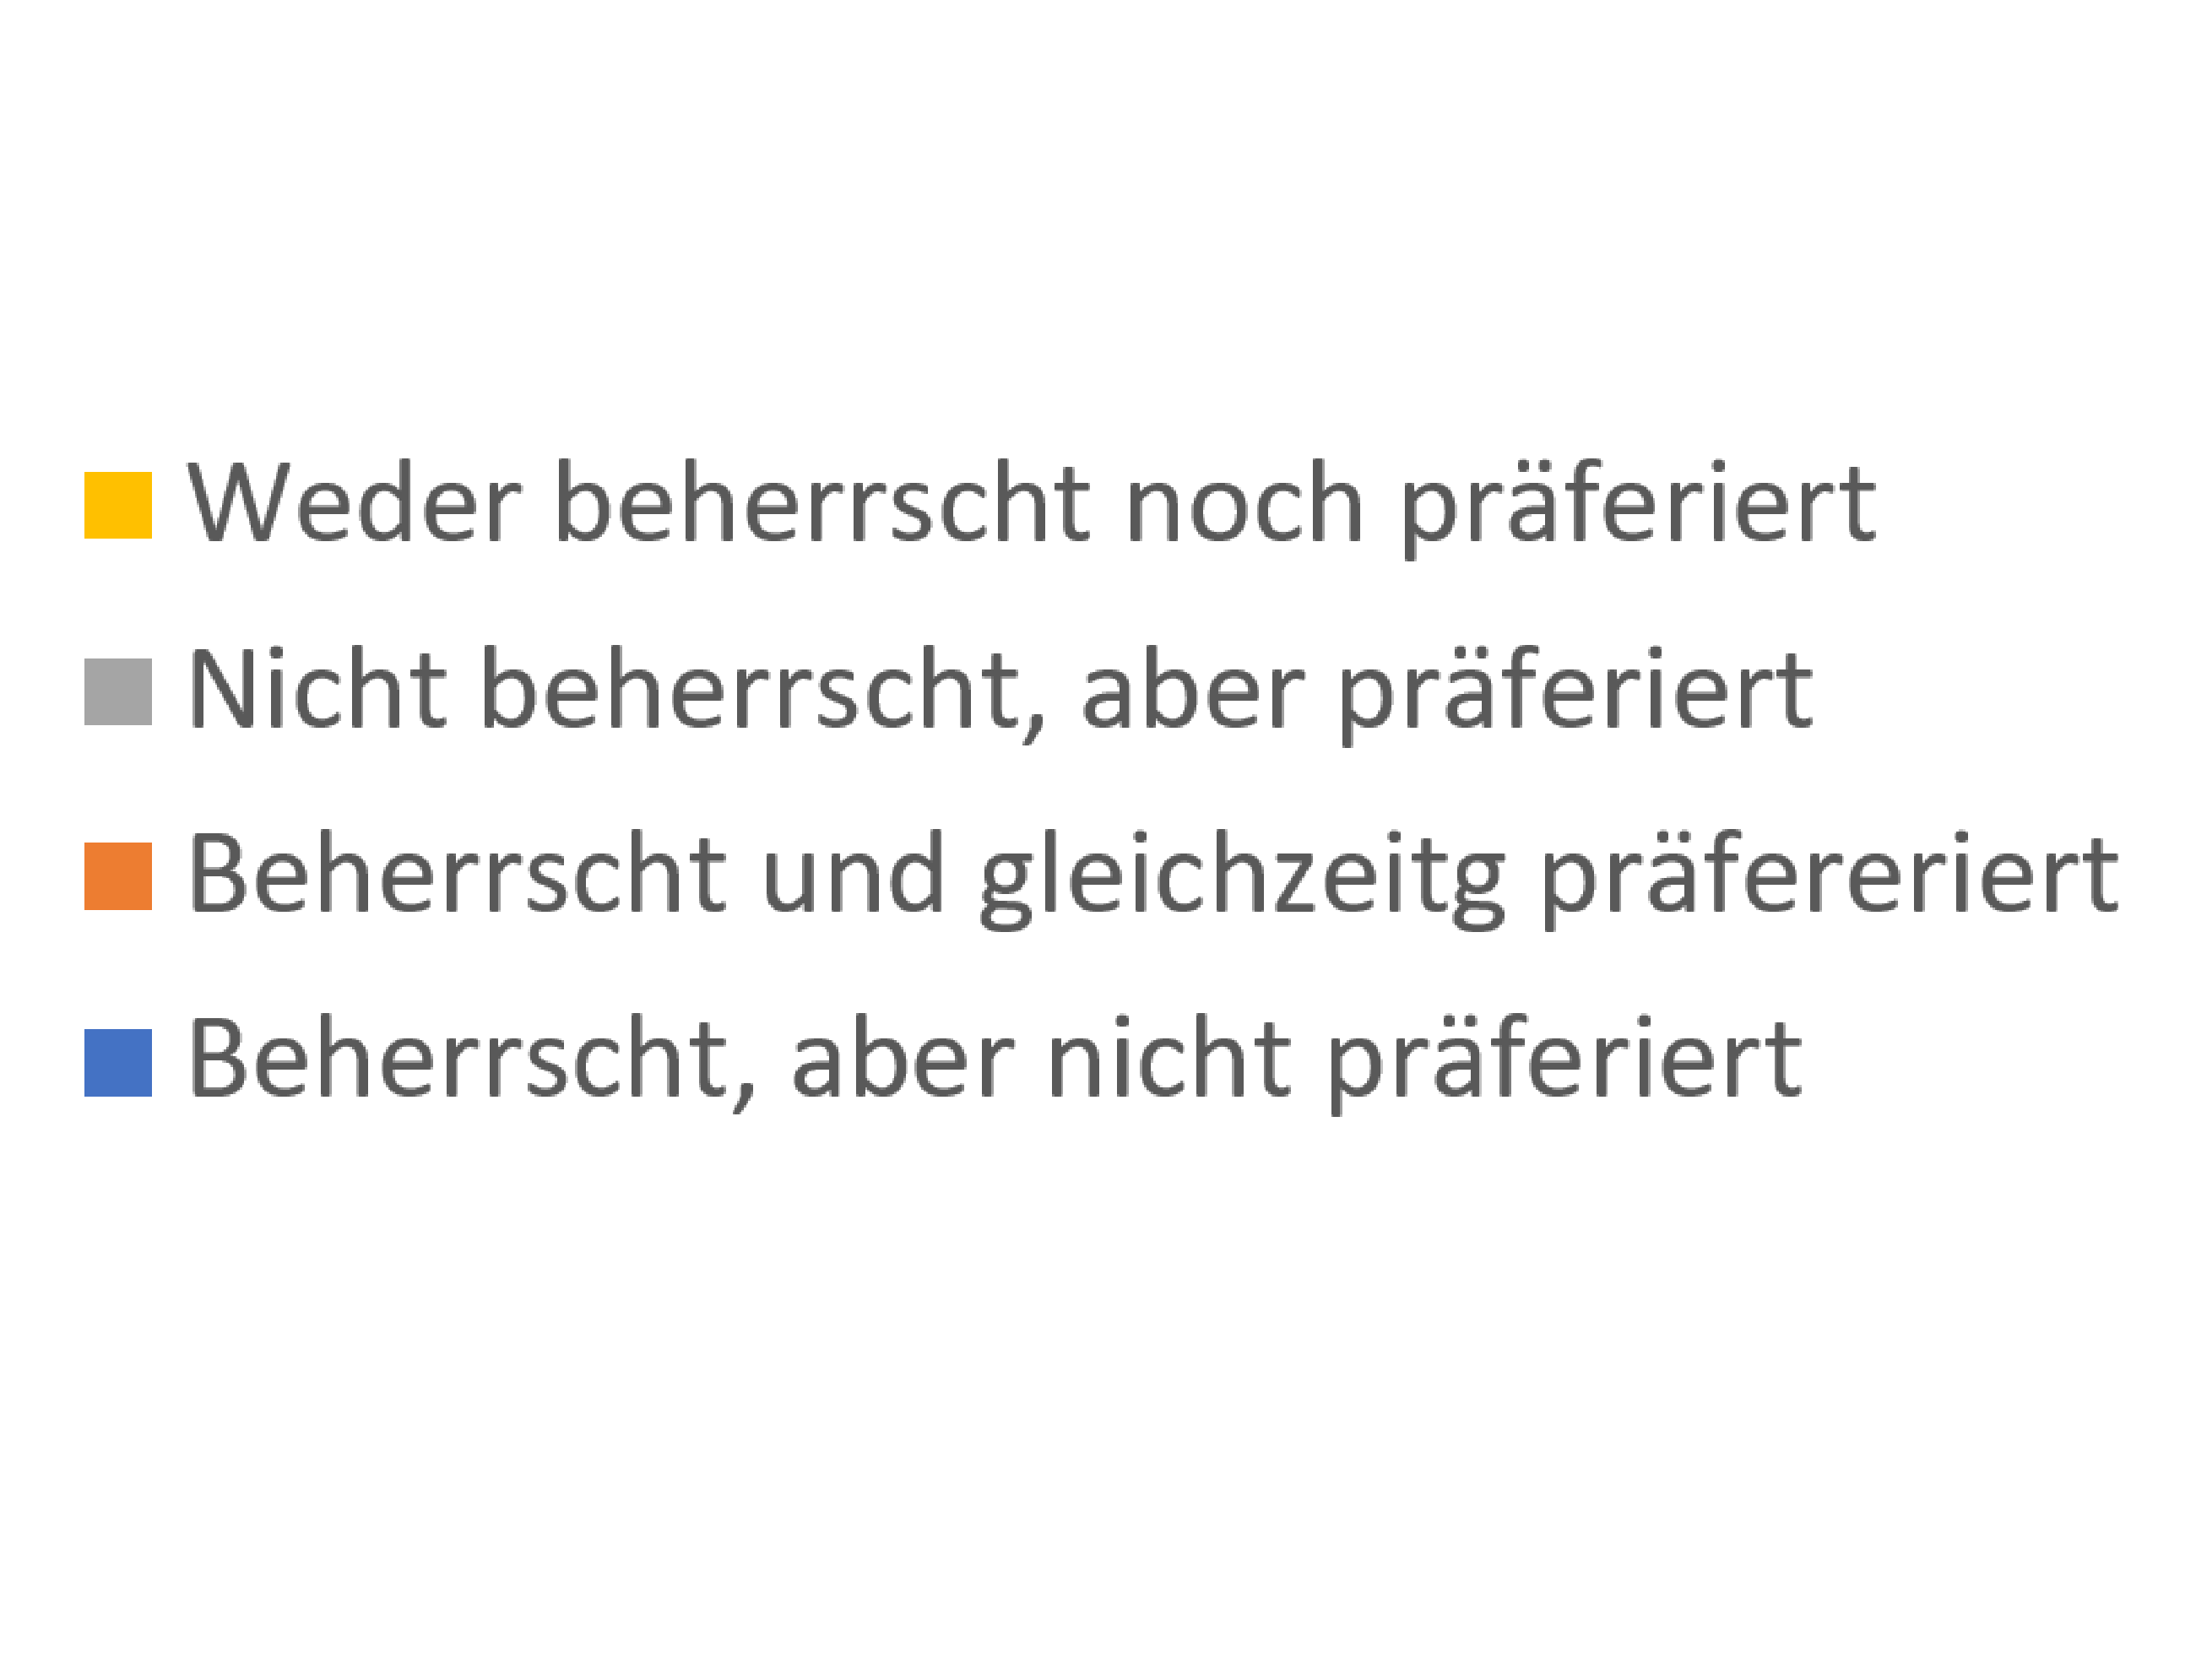
\includegraphics[width = 0.4\textwidth]{gfx/projekt-detail-legende.png}}
	
	\caption{Anteil an Mitarbeitern, welche die in den jeweiligen Beispielprojektpositionen gesuchten Fähigkeiten beherrschen bzw. präferieren}
\label{fig:ergebnisse:analyse:abb6}
\end{figure}

In Abbildung \ref{fig:ergebnisse:analyse:abb6} ist zu erkennen, dass im Durchschnitt 31 Prozent der gesuchten Fähigkeiten jedes Projekts von mindestens der Hälfte aller Mitarbeiter beherrscht werden. Für die übrigen 69 Prozent der Kompetenzen ist anschließend ein zumeist lineares Absinken der Angestellten zu beobachten, welche über diese Fähigkeiten verfügen. Wie stark die Abnahme ist, unterscheidet sich zwischen den einzelnen Projektpositionen stark. So beherrschen bei Projektposition E 17 Prozent aller Mitarbeiter mindestens eine Fähigkeit. Bei den Projektpositionen A und C werden dagegen 17 Prozent der gesuchten Fähigkeiten von keinem einzigen Angestellten beherrscht. In den Grafiken aus Abbildung \ref{fig:ergebnisse:analyse:abb6} ist außerdem zu beobachten, dass keine Kompetenz gesucht wird, welche kein einziger Angestellter in der Umfrage als Präferenz angegebene hat.

\section{Ergebnisse der Fallstudie}
\label{ch:ergebnisse:fallstudie}

\subsection{Erwartete Zufriedenheit der Projektmitarbeiter}
\label{ch:ergebnisse:fallstudie:umfrageMitarbeiter}
In der in Kapitel \ref{ch:methodik:evaluation} vorgestellten Umfrage wurde erhoben, welche Zufriedenheit die Mitarbeiter der EXXETA AG mit Tätigkeiten auf den Projektpositionen aus Abbildung \ref{fig:methodik:evaluation:abb2} prognostizieren. Die Ergebnisse sind in Abbildung \ref{fig:ergebnisse:fallstudie:abb1} dargestellt.

\begin{figure}[h]
	\centering
	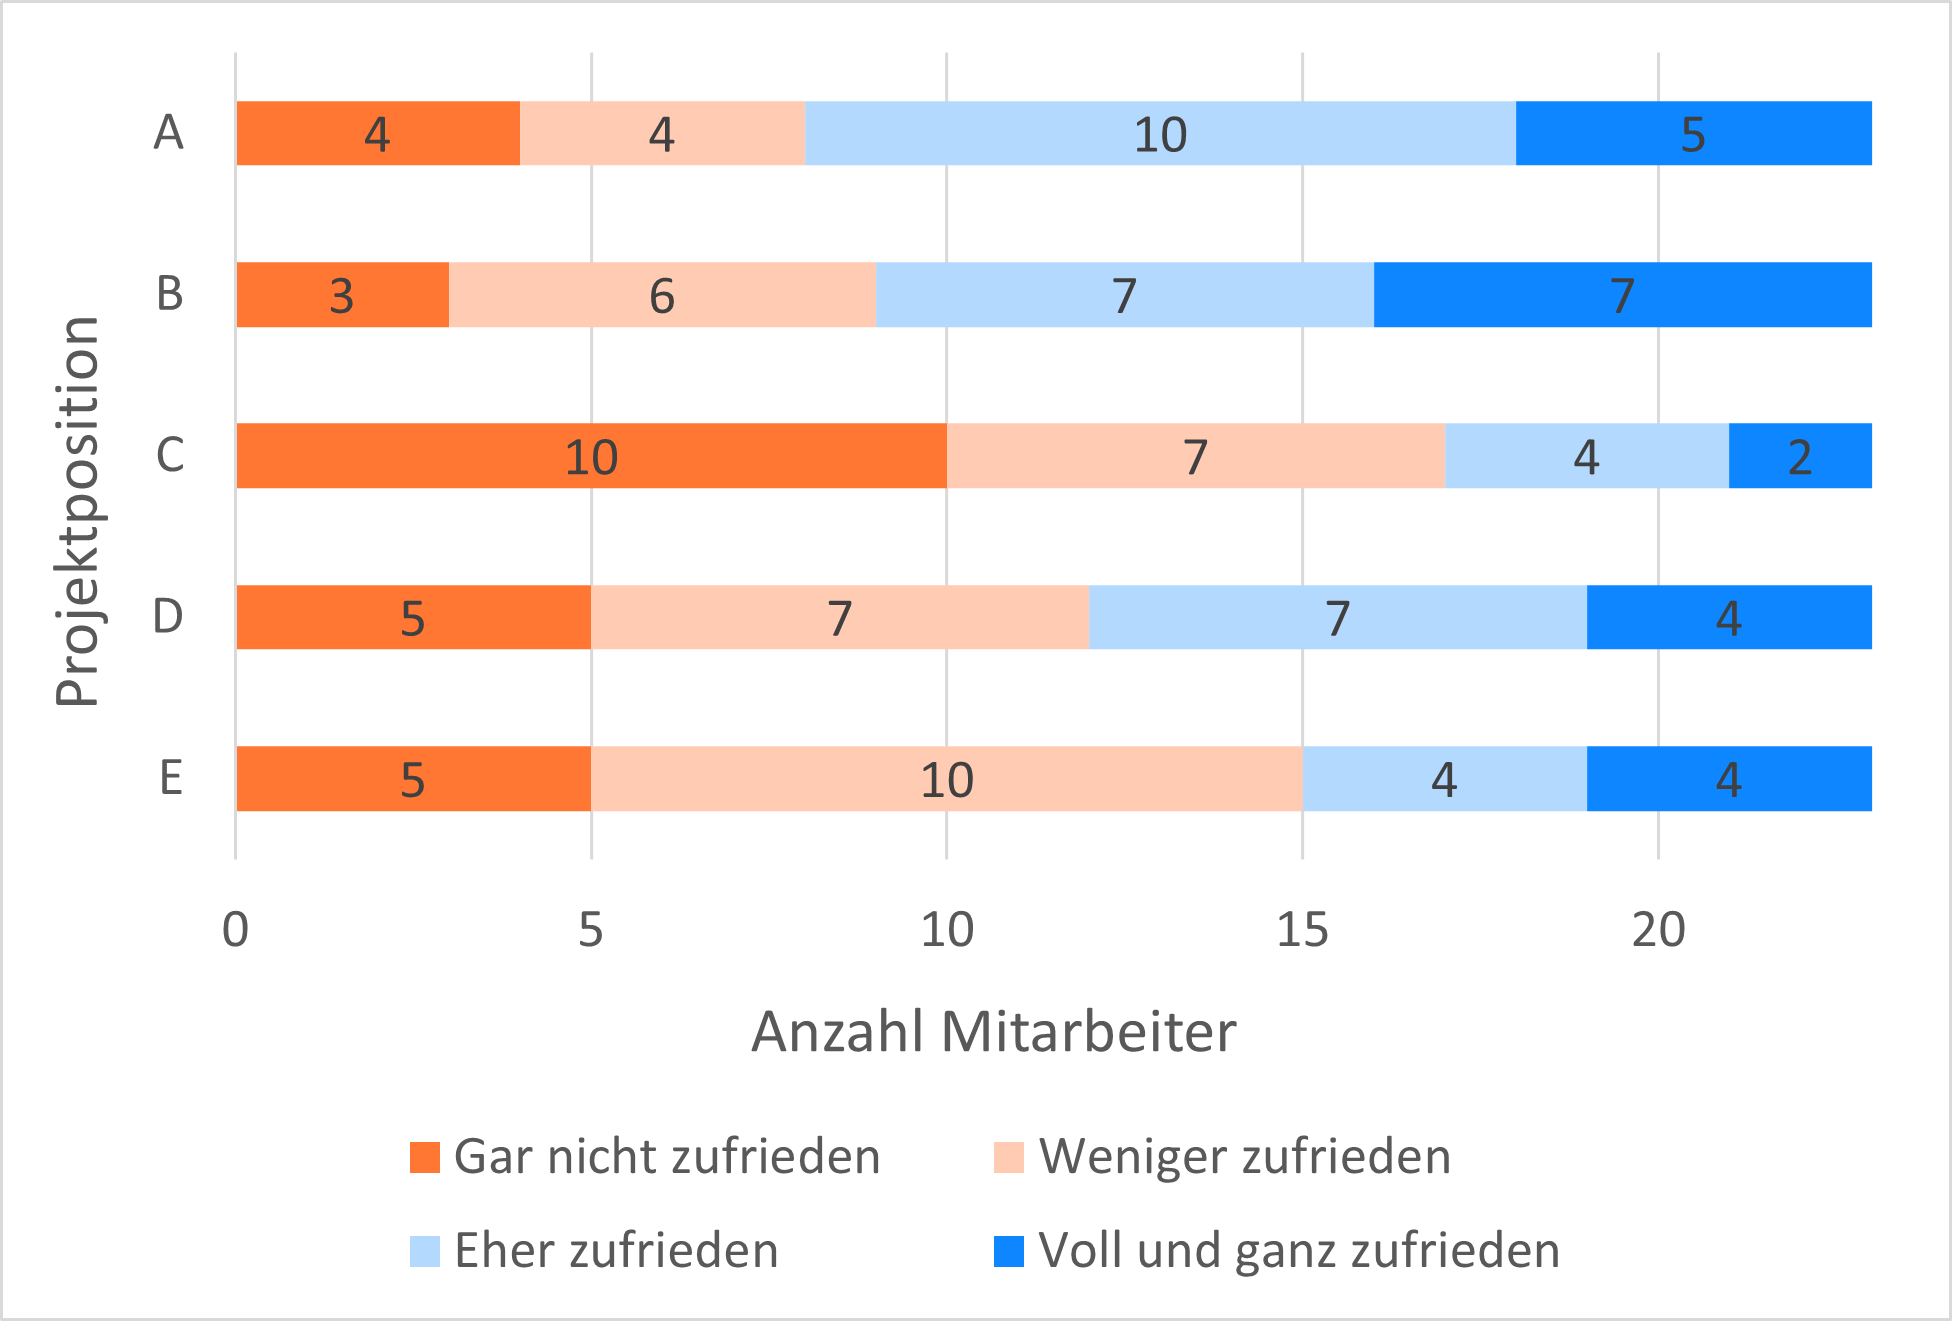
\includegraphics[width=1\textwidth]{gfx/mitarbeiter-zufriedenheit-umfrage.png}
	\caption{Anzahl an Mitarbeitern, welche zufrieden bzw. unzufrieden mit der Tätigkeit auf den jeweiligen Beispielprojektpositionen wären}
	\label{fig:ergebnisse:fallstudie:abb1}
\end{figure}

In Abbildung \ref{fig:ergebnisse:fallstudie:abb1} ist zu erkennen, dass die Mitarbeiter überwiegend eine hohe Zufriedenheit mit den Projektpositionen A und B prognostizieren. Mit einer Tätigkeit auf den Projektpositionen C und E zeigen sich die Angestellten eher unzufrieden. Projektposition D stehen die Mitarbeiter gespalten gegenüber, sodass etwa die Hälfte der Befragten zufrieden und die andere Hälfte unzufrieden mit dieser Tätigkeit wäre.

Abbildung \ref{fig:ergebnisse:analyse:abb7} zeigt, für wie viele der 23 befragten Mitarbeiter der bilaterale Empfehlungsansatz gegenüber dem unilateralen Vorgehen für eine höhere Zufriedenheit seitens der Mitarbeiter sorgte. Wie in Kapitel \ref{ch:methodik:evaluation} beschrieben, entsteht eine höhere Zufriedenheit mit den Projekttätigkeiten, wenn das bilaterale System die Angestellten bei einer prognostizierten Zufriedenheit höher und bei einer erwarteten Unzufriedenheit niedriger positioniert als die unilaterale Anwendung.

\begin{figure}[h]
	\centering
	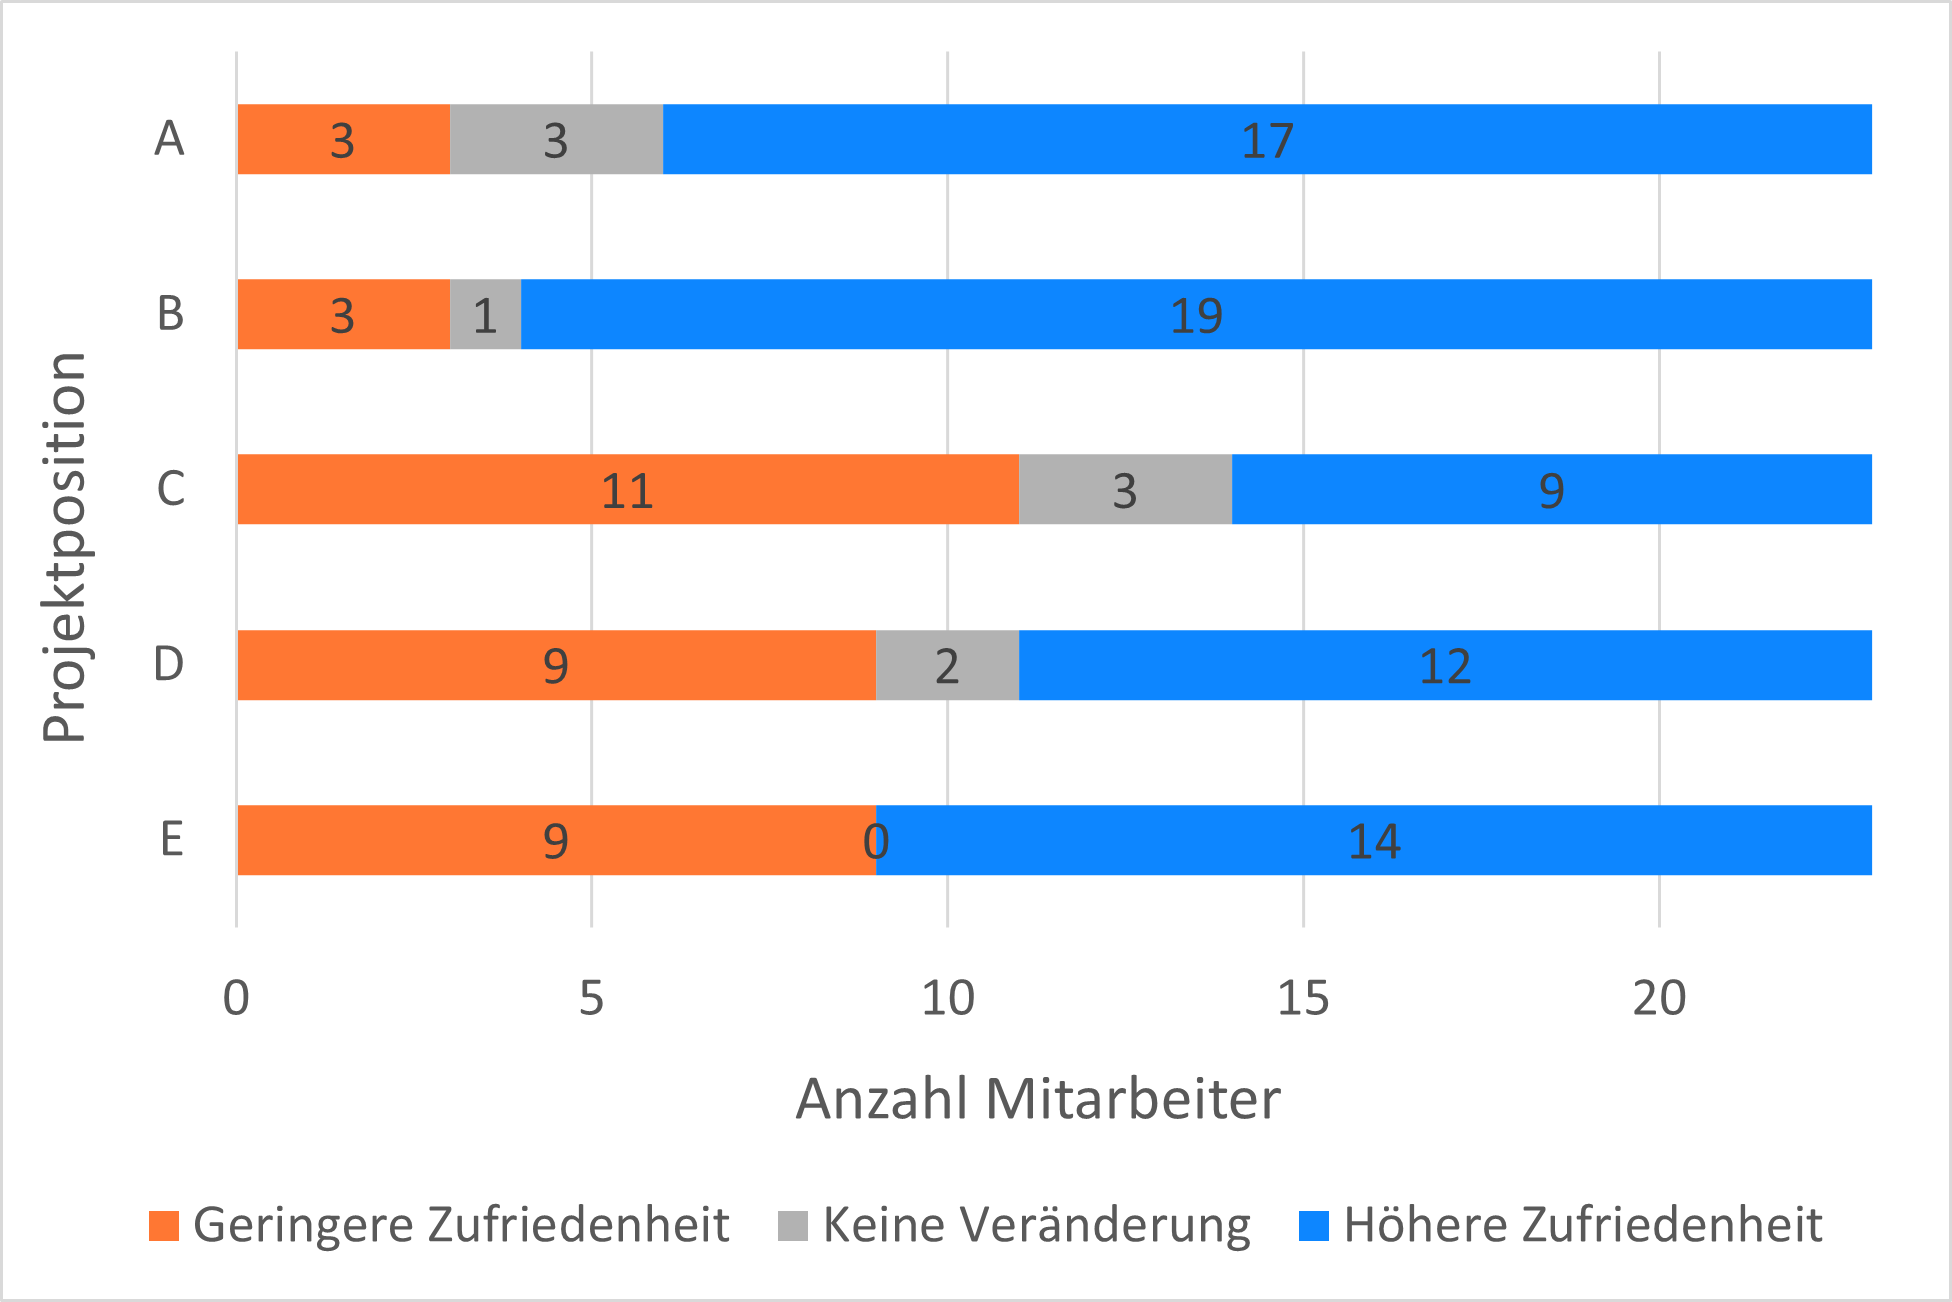
\includegraphics[width=1\textwidth]{gfx/zufriedenheit-projekte.png}	
	\caption{Ergebnisse des bilateralen Empfehlungsansatzes im Vergleich zum unilateralen Vorgehen hinsichtlich der Mitarbeiterzufriedenheit}
	\label{fig:ergebnisse:analyse:abb7}
\end{figure}

In Abbildung \ref{fig:ergebnisse:analyse:abb7} ist zu erkennen, dass der bilaterale Empfehlungsansatz einen Großteil der Angestellten für die Projektpositionen A und B zugunsten einer höheren Zufriedenheit positionierte. Bei den Projektpositionen D und E sind erreiche das bilaterale Vorschlagsverfahren für knapp über die Hälfte der Mitarbeiter eine höhere Zufriedenheit. Bei Projektposition C konnte dagegen der unilaterale Empfehlungsansatz für den Großteil der Angestellten eine höhere Zufriedenheit erzielen.

\subsection{Prognostizierte Arbeitsleistung der Projektmanager}
\label{ch:ergebnisse:fallstudie:arbeitsleistung}
An der Umfrage unter den Projektmanagern haben N=\anzPM Personen teilgenommen. Fünf der Teilnehmer sind im Bereich \acl{JES} tätig. Eine Person stammt aus einer anderen Abteilung, welche ähnliche Technologien bei der Projekttätigkeit einsetzt.

Abbildung \ref{fig:ergebnisse:fallstudie:arbeitsleistung:abb1} zeigt, von den Mitarbeitern der Listen welches Empfehlungsansatzes die Projektmanager eine höhere Arbeitsleistung erwarten.

\begin{figure}[h]
	\centering
	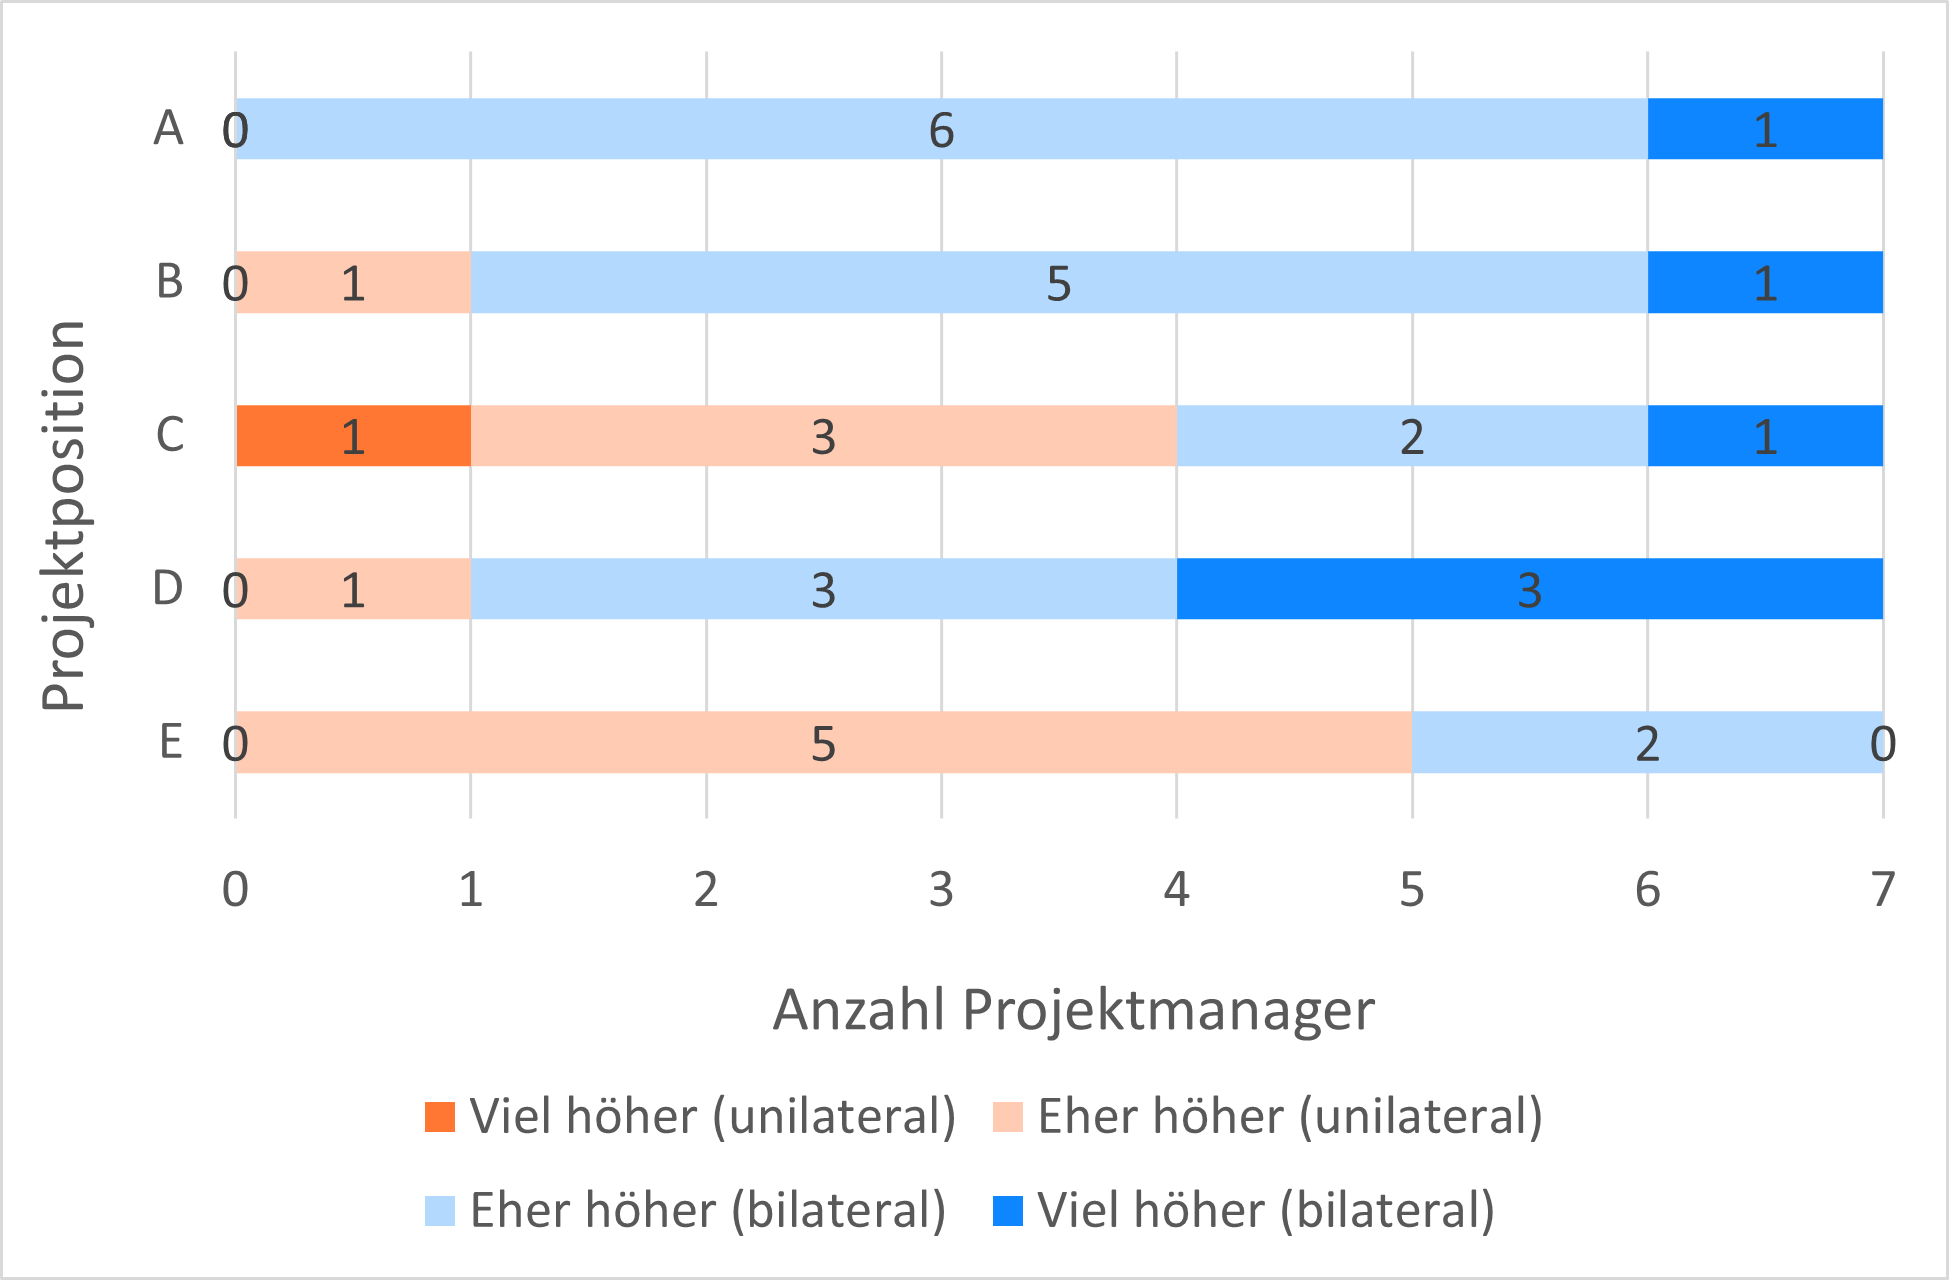
\includegraphics[width=1\textwidth]{gfx/ergebnisse-projektmanager-arbeitsleistung.png}	
	\caption{Ergebnisse der Umfrage unter den Projektmanager hinsichtlich der erwarteten Arbeitsleistung der Mitarbeiter}
	\label{fig:ergebnisse:fallstudie:arbeitsleistung:abb1}
\end{figure}

An den Ergebnissen aus Abbildung \ref{fig:ergebnisse:fallstudie:arbeitsleistung:abb1} ist zu erkennen, dass die Projektmanager in sämtlichen Projektpositionen 

% TODO: KURVEN
\shorthandon{"}
